\chapter{Eigenvalues, Eigenvectors and Symmetric Matrices}\label{ch:eigen}

\begin{chapterintro}
Pluck a guitar string and you hear a note. Touch the string lightly at its midpoint and you hear the octave above. A string fixed at both ends cannot vibrate in any pattern it likes and still keep its shape as it oscillates. It has a list of special shapes, the harmonics, each of which oscillates at its own frequency. Any other motion is a mixture of these. The harmonics and their frequencies are the simplest example of the idea at the center of this chapter: an \emph{eigenvalue problem}. A linear operation (here, the restoring force of the string) acts on most shapes by changing them into different shapes, but on a few special shapes it acts by simple multiplication. Those shapes are eigenvectors, and the multipliers are eigenvalues.

In quantum mechanics this idea is the whole story. The allowed energies of a particle trapped in a potential are the eigenvalues of an operator called the Hamiltonian, and the corresponding states are its eigenvectors. On a computer the Hamiltonian becomes a large matrix, and finding energy levels means finding eigenvalues of that matrix. The matrices that arise from physical energies are \emph{symmetric} (or, with complex entries, \emph{Hermitian}), and for those we will prove two facts that physics depends on: their eigenvalues are real and their eigenvectors are mutually perpendicular. We will also see what goes wrong for matrices that are not symmetric: eigenvalues can become complex and eigenvectors stop being perpendicular.

Where this shows up in the paper \cite{soniR1}: the phrase ``spectrum of a self-adjoint operator'' in the first sentence of Sec.~I is a statement about real eigenvalues; Sec.~II~B computes energy levels as eigenvalues of a ``symmetric tridiagonal matrix'' with ``eigenpairs from LAPACK''; and Sec.~II~E (iii) and Sec.~V diagonalize non-Hermitian matrices exactly and match their eigenvectors to reference states ``by overlap''. By the end of this chapter you will understand each of those phrases, and you will be able to compute the levels of a particle in a box on your own computer.
\end{chapterintro}

\begin{prerequisites}
\item Chapter~\ref{ch:complex}: complex numbers, the conjugate $z^*$, the modulus $\abs{z}$, Euler's formula $e^{i\theta}=\cos\theta+i\sin\theta$.
\item Chapter~\ref{ch:linear-algebra}: vectors in $n$ dimensions (real and complex), the inner product, norm and orthogonality; matrix multiplication, transpose $A^\top$ and conjugate transpose $A^\dagger$; the identity $I$ and the inverse; determinants of $2\times2$ and $3\times3$ matrices and their stated properties; the fact that a square matrix $B$ is invertible exactly when $\det B\ne0$, exactly when $Bv=0$ has only the solution $v=0$; linear independence and bases; functions sampled on a grid as vectors.
\item First-year physics: standing waves on a string fixed at both ends, harmonics \cite{hrw}; Taylor expansion of a smooth function.
\end{prerequisites}

%==========================================================
\section{Special directions: the eigenvalue equation}\label{sec:eigen-equation}

Recall from Chapter~\ref{ch:linear-algebra} that an $n\times n$ matrix $A$ is a machine that takes an $n$-component vector $v$ and returns another $n$-component vector $Av$. In two dimensions you can picture this: draw the arrow $v$, apply $A$, draw the arrow $Av$. In general $Av$ points in a different direction from $v$ and has a different length. Some matrices, though, have special directions along which they act very simply: they only stretch or shrink (or flip) the arrow, never turn it.

Take the matrix
\begin{equation}
A=\begin{pmatrix}2&1\\1&2\end{pmatrix}.
\label{eq:eigen-A21}
\end{equation}
Apply it to $v=(1,0)^\top$ (we write column vectors as transposed rows to save space):
\begin{equation}
A\begin{pmatrix}1\\0\end{pmatrix}=\begin{pmatrix}2\cdot1+1\cdot0\\1\cdot1+2\cdot0\end{pmatrix}=\begin{pmatrix}2\\1\end{pmatrix}.
\end{equation}
The arrow has been turned: $(1,0)$ points along the horizontal axis, $(2,1)$ points up and to the right. Now apply $A$ to $u=(1,1)^\top$:
\begin{equation}
A\begin{pmatrix}1\\1\end{pmatrix}=\begin{pmatrix}2+1\\1+2\end{pmatrix}=\begin{pmatrix}3\\3\end{pmatrix}=3\begin{pmatrix}1\\1\end{pmatrix}.
\end{equation}
This arrow was not turned at all; it was stretched by a factor of $3$. Try $w=(1,-1)^\top$:
\begin{equation}
A\begin{pmatrix}1\\-1\end{pmatrix}=\begin{pmatrix}2-1\\1-2\end{pmatrix}=\begin{pmatrix}1\\-1\end{pmatrix}=1\cdot\begin{pmatrix}1\\-1\end{pmatrix}.
\end{equation}
This arrow is left exactly as it was: stretched by the factor $1$. \Cref{fig:eigen-stretch} shows what $A$ does to every unit vector at once: it turns the unit circle into an ellipse whose long axis lies along $(1,1)$ with half-length $3$ and whose short axis lies along $(1,-1)$ with half-length $1$.

\begin{figure}[htbp]\centering
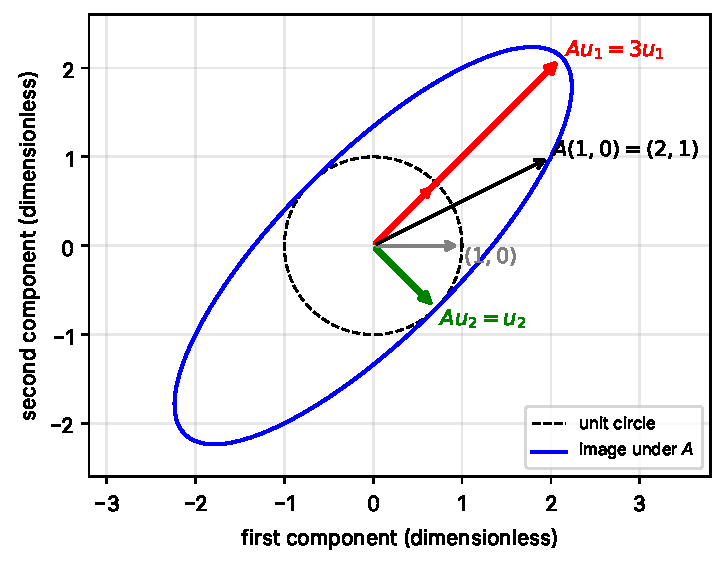
\includegraphics[width=0.85\linewidth]{figs/eigen_stretch.pdf}
\caption{The matrix $A$ of Eq.~\eqref{eq:eigen-A21} applied to every unit vector. The dashed unit circle is mapped to the solid ellipse. The two eigen-directions (red and green) are only stretched, by the eigenvalues $3$ and $1$; the generic vector $(1,0)$ (gray) is turned into $(2,1)$ (black). All quantities are dimensionless.}
\label{fig:eigen-stretch}
\end{figure}

\paragraph{Definition.} Let $A$ be an $n\times n$ matrix, with real or complex entries. A number $\lambda$ (real or complex) is an \emph{eigenvalue} of $A$ if there is a \emph{nonzero} vector $v$ such that
\begin{equation}
\boxed{Av=\lambda v.}
\label{eq:eigen-def}
\end{equation}
Any such nonzero $v$ is an \emph{eigenvector} belonging to $\lambda$. The pair $(\lambda,v)$ is called an \emph{eigenpair}. The set of all eigenvalues of $A$ is its \emph{spectrum}. (``Eigen'' is German for ``own'' or ``characteristic'': these are the matrix's own special values.)

Two remarks make the definition precise.

First, the zero vector is excluded on purpose. For $v=0$ we have $A0=0=\lambda\cdot0$ for every number $\lambda$, which would make every number an eigenvalue and the idea useless.

Second, an eigenvector is really a \emph{direction}, not a single vector. If $Av=\lambda v$ and $a$ is any nonzero number, then
\begin{equation}
A(av)=a(Av)=a(\lambda v)=\lambda(av),
\end{equation}
where the first step uses linearity of matrix multiplication (Chapter~\ref{ch:linear-algebra}). So $av$ is also an eigenvector with the same eigenvalue. It is common to pick the representative of unit length, $\norm{v}=1$; this is called \emph{normalizing} the eigenvector. Even then the sign (for real vectors) or a phase factor $e^{i\alpha}$ (for complex vectors) remains free.

For the matrix \eqref{eq:eigen-A21}, normalized eigenvectors are
\begin{equation}
u_1=\frac{1}{\sqrt2}\begin{pmatrix}1\\1\end{pmatrix}\ (\lambda_1=3),\qquad
u_2=\frac{1}{\sqrt2}\begin{pmatrix}1\\-1\end{pmatrix}\ (\lambda_2=1).
\label{eq:eigen-A21-vecs}
\end{equation}
Notice something: $u_1\cdot u_2=\tfrac12(1\cdot1+1\cdot(-1))=0$. The two eigenvectors are perpendicular. That is not an accident; it happens because $A$ is symmetric ($A_{12}=A_{21}$), and we will prove in \cref{sec:eigen-hermitian} that it always happens for symmetric matrices.

\paragraph{The physical picture.} Think of the matrix as a rule that says how a system responds. For a string, the ``vector'' is the list of displacements at many points, and the matrix gives the restoring force at each point. A harmonic is a shape for which the restoring force at every point is proportional to the displacement there, with the same constant of proportionality everywhere. Then every point oscillates like a simple harmonic oscillator with the same frequency, and the shape is preserved. The constant of proportionality is the eigenvalue. We will make this precise in \cref{sec:eigen-ode}.

\begin{checkpoint}
Suppose $Av=3v$ for a nonzero vector $v$. What is $A(5v)$? What is $A(A v)$?
\end{checkpoint}
\checkanswer{$A(5v)=5Av=15v=3(5v)$, so $5v$ is an eigenvector with the same eigenvalue $3$. Also $A(Av)=A(3v)=3Av=9v$: applying $A$ twice multiplies by $3^2$.}

\begin{keyideas}
\item An eigenpair $(\lambda,v)$ of a square matrix $A$ satisfies $Av=\lambda v$ with $v\ne0$, Eq.~\eqref{eq:eigen-def}.
\item Eigenvectors are directions that $A$ stretches, shrinks or flips without turning; any nonzero multiple of an eigenvector is again an eigenvector with the same eigenvalue.
\item Normalizing ($\norm{v}=1$) fixes the length but leaves a sign or phase free.
\end{keyideas}

%==========================================================
\section{The characteristic polynomial}\label{sec:eigen-charpoly}

Guessing eigenvectors, as we did above, does not scale. We need a systematic way to find all eigenvalues. Here it is.

\paragraph{Derivation.} Write $\lambda v$ as $\lambda I v$, where $I$ is the $n\times n$ identity matrix (ones on the diagonal, zeros elsewhere), so that Eq.~\eqref{eq:eigen-def} becomes
\begin{align}
Av&=\lambda Iv\\
Av-\lambda Iv&=0\\
(A-\lambda I)v&=0.\quad\text{(distributive law for matrices)}
\label{eq:eigen-homog}
\end{align}
So $\lambda$ is an eigenvalue exactly when the matrix $B=A-\lambda I$ sends some \emph{nonzero} vector to zero. Recall from Chapter~\ref{ch:linear-algebra} that a square matrix $B$ has a nonzero solution of $Bv=0$ if and only if $\det B=0$. Therefore
\begin{equation}
\boxed{\lambda\ \text{is an eigenvalue of }A\iff\det(A-\lambda I)=0.}
\label{eq:eigen-chareq}
\end{equation}
Equation \eqref{eq:eigen-chareq} is the \emph{characteristic equation}. When you expand the determinant, each entry on the diagonal of $A-\lambda I$ contains $\lambda$ once, so $\det(A-\lambda I)$ is a polynomial in $\lambda$ of degree $n$ (the highest power comes from the product of the $n$ diagonal entries). It is called the \emph{characteristic polynomial} of $A$, and we write $p_A(\lambda)=\det(A-\lambda I)$.

Once you have an eigenvalue $\lambda$, you find its eigenvectors by solving the linear system $(A-\lambda I)v=0$ by elimination, exactly as in Chapter~\ref{ch:linear-algebra}. Because $\det(A-\lambda I)=0$, elimination will always produce at least one row of zeros, leaving at least one free component that you may choose.

\begin{beyond}
\textbf{Taken on trust: the fundamental theorem of algebra.} Every polynomial of degree $n\ge1$ with complex coefficients has exactly $n$ complex roots when each root is counted as many times as it is repeated. Hence every $n\times n$ matrix has exactly $n$ eigenvalues counted with repetition, though some may be complex even when all entries of $A$ are real, and some may coincide. The proof needs complex analysis and is given in many texts, for example \cite{rhb}. We use only the statement.
\end{beyond}

The number of times a value $\lambda$ appears as a root of $p_A$ is its \emph{algebraic multiplicity}. An eigenvalue of multiplicity one is called \emph{simple} or \emph{nondegenerate}; one of multiplicity two or more is \emph{degenerate}.

\subsection{The $2\times2$ case in general}

For a general $2\times2$ matrix
\begin{equation}
A=\begin{pmatrix}a&b\\c&d\end{pmatrix},
\end{equation}
we have
\begin{equation}
A-\lambda I=\begin{pmatrix}a-\lambda&b\\c&d-\lambda\end{pmatrix},
\end{equation}
and the $2\times2$ determinant rule ``product of diagonal minus product of off-diagonal'' gives
\begin{align}
p_A(\lambda)&=(a-\lambda)(d-\lambda)-bc\\
&=ad-a\lambda-d\lambda+\lambda^2-bc\\
&=\lambda^2-(a+d)\lambda+(ad-bc).
\label{eq:eigen-char2}
\end{align}
The coefficient $a+d$ is the sum of the diagonal entries, called the \emph{trace}, $\operatorname{tr}A$. The constant $ad-bc$ is $\det A$. So
\begin{equation}
p_A(\lambda)=\lambda^2-(\operatorname{tr}A)\lambda+\det A.
\label{eq:eigen-char2b}
\end{equation}
If the two roots are $\lambda_1$ and $\lambda_2$, then $p_A(\lambda)=(\lambda-\lambda_1)(\lambda-\lambda_2)=\lambda^2-(\lambda_1+\lambda_2)\lambda+\lambda_1\lambda_2$. Comparing coefficients of $\lambda$ and of $\lambda^0$ with Eq.~\eqref{eq:eigen-char2b}:
\begin{equation}
\lambda_1+\lambda_2=\operatorname{tr}A,\qquad \lambda_1\lambda_2=\det A.
\label{eq:eigen-trdet}
\end{equation}
These two relations are handy checks on any eigenvalue calculation. (For $n\times n$ matrices the same two facts hold. The determinant part follows in one line. By the fundamental theorem of algebra (box above), and because the highest power of $\lambda$ in $\det(A-\lambda I)$ is $(-\lambda)^n$, coming from the product of the diagonal entries, we can write $p_A(\lambda)=(\lambda_1-\lambda)(\lambda_2-\lambda)\cdots(\lambda_n-\lambda)$, with each eigenvalue repeated according to its multiplicity. Setting $\lambda=0$ gives $\det A=\lambda_1\lambda_2\cdots\lambda_n$. The trace part, $\lambda_1+\dots+\lambda_n=\operatorname{tr}A$, we state without proof; it follows by comparing the coefficients of $\lambda^{n-1}$ on the two sides, see \cite{strang}. We use the factorization in \cref{sec:eigen-numerics} and both $n\times n$ facts in the answer to Problem~31.)

The quadratic formula applied to Eq.~\eqref{eq:eigen-char2b} gives
\begin{equation}
\lambda_\pm=\frac{\operatorname{tr}A\pm\sqrt{(\operatorname{tr}A)^2-4\det A}}{2}.
\label{eq:eigen-quadratic}
\end{equation}

For the matrix \eqref{eq:eigen-A21}: $\operatorname{tr}A=4$, $\det A=4-1=3$, so $p_A(\lambda)=\lambda^2-4\lambda+3=(\lambda-3)(\lambda-1)$, confirming the eigenvalues $3$ and $1$.

\begin{sample}{Eigenpairs of a non-symmetric $2\times2$ matrix}
Find all eigenvalues and eigenvectors of $B=\begin{pmatrix}4&1\\2&3\end{pmatrix}$ and check whether the eigenvectors are perpendicular.

\textbf{Step 1: characteristic polynomial.} $\operatorname{tr}B=4+3=7$ and $\det B=4\cdot3-1\cdot2=10$, so by Eq.~\eqref{eq:eigen-char2b}
\[
p_B(\lambda)=\lambda^2-7\lambda+10=(\lambda-5)(\lambda-2).
\]
(Check the factorization: $(\lambda-5)(\lambda-2)=\lambda^2-7\lambda+10$.)

\textbf{Step 2: eigenvector for $\lambda=5$.} Solve $(B-5I)v=0$:
\[
\begin{pmatrix}-1&1\\2&-2\end{pmatrix}\begin{pmatrix}v_1\\v_2\end{pmatrix}=0.
\]
The first row says $-v_1+v_2=0$, so $v_2=v_1$. The second row says $2v_1-2v_2=0$, the same condition (as it must be, since the determinant is zero). Choosing $v_1=1$: $v=(1,1)^\top$.

\textbf{Step 3: eigenvector for $\lambda=2$.} Solve $(B-2I)v=0$:
\[
\begin{pmatrix}2&1\\2&1\end{pmatrix}\begin{pmatrix}v_1\\v_2\end{pmatrix}=0,
\]
so $2v_1+v_2=0$, $v_2=-2v_1$. Choosing $v_1=1$: $v=(1,-2)^\top$.

\textbf{Step 4: check.} $B(1,1)^\top=(4+1,2+3)^\top=(5,5)^\top=5(1,1)^\top$ and $B(1,-2)^\top=(4-2,2-6)^\top=(2,-4)^\top=2(1,-2)^\top$. Also $\lambda_1+\lambda_2=7=\operatorname{tr}B$ and $\lambda_1\lambda_2=10=\det B$.

\textbf{Step 5: perpendicular?} $(1,1)\cdot(1,-2)=1-2=-1\ne0$.

\[
\boxed{\lambda=5,\ v=(1,1)^\top;\quad \lambda=2,\ v=(1,-2)^\top;\quad\text{eigenvectors not perpendicular.}}
\]
The matrix is not symmetric ($B_{12}=1\ne B_{21}=2$), and its eigenvectors are not orthogonal.
\end{sample}

\subsection{The $3\times3$ case}

For a $3\times3$ matrix the characteristic polynomial is cubic. You expand $\det(A-\lambda I)$ along the first row (the cofactor expansion of Chapter~\ref{ch:linear-algebra}). The following example is important, because the same matrix (in a bigger size) will be our model of the second derivative in \cref{sec:eigen-second-derivative}.

\begin{sample}{The three-point second-difference matrix}
Find the eigenvalues and eigenvectors of
\[
D_3=\begin{pmatrix}2&-1&0\\-1&2&-1\\0&-1&2\end{pmatrix}.
\]

\textbf{Step 1: set up.} Write $a=2-\lambda$ to keep the algebra short. Then
\[
D_3-\lambda I=\begin{pmatrix}a&-1&0\\-1&a&-1\\0&-1&a\end{pmatrix}.
\]

\textbf{Step 2: expand along the first row.} The cofactor expansion gives
\[
\det(D_3-\lambda I)=a\det\begin{pmatrix}a&-1\\-1&a\end{pmatrix}-(-1)\det\begin{pmatrix}-1&-1\\0&a\end{pmatrix}+0.
\]
The two $2\times2$ determinants are $a\cdot a-(-1)(-1)=a^2-1$ and $(-1)a-(-1)\cdot0=-a$. So
\[
\det(D_3-\lambda I)=a(a^2-1)+(-a)=a^3-a-a=a^3-2a=a(a^2-2).
\]

\textbf{Step 3: roots.} $a(a^2-2)=0$ gives $a=0$ or $a=\pm\sqrt2$. Since $\lambda=2-a$:
\[
\lambda=2-\sqrt2\approx0.585786,\qquad \lambda=2,\qquad \lambda=2+\sqrt2\approx3.414214.
\]

\textbf{Step 4: eigenvectors.} For each eigenvalue solve $(D_3-\lambda I)v=0$, i.e.\ the three equations $av_1-v_2=0$, $-v_1+av_2-v_3=0$, $-v_2+av_3=0$.

From the first, $v_2=av_1$. From the third, $v_2=av_3$. If $a\ne0$, these give $v_3=v_1$. Then the second equation, $-v_1+a(av_1)-v_1=(a^2-2)v_1=0$, holds automatically because $a^2=2$. Choosing $v_1=1$:
\begin{itemize}
\item $a=\sqrt2$ ($\lambda=2-\sqrt2$): $v=(1,\sqrt2,1)^\top$;
\item $a=-\sqrt2$ ($\lambda=2+\sqrt2$): $v=(1,-\sqrt2,1)^\top$.
\end{itemize}
If $a=0$ ($\lambda=2$), the first and third equations give $v_2=0$, and the second gives $-v_1-v_3=0$, so $v_3=-v_1$: $v=(1,0,-1)^\top$.

\textbf{Step 5: check orthogonality.} $(1,\sqrt2,1)\cdot(1,0,-1)=1-1=0$; $(1,\sqrt2,1)\cdot(1,-\sqrt2,1)=1-2+1=0$; $(1,0,-1)\cdot(1,-\sqrt2,1)=1-1=0$.

\[
\boxed{\lambda=2-\sqrt2,\ 2,\ 2+\sqrt2;\quad v=(1,\sqrt2,1),\ (1,0,-1),\ (1,-\sqrt2,1).}
\]
The matrix is symmetric, and again the eigenvectors are mutually perpendicular. Look at the shapes: the first has no change of sign, the second has one, the third has two. Keep this in mind; it is the discrete version of the harmonics of a string.
\end{sample}

\subsection{Two easy families: diagonal and triangular matrices}

If $A$ is \emph{diagonal}, $A=\operatorname{diag}(d_1,\dots,d_n)$, then $A-\lambda I=\operatorname{diag}(d_1-\lambda,\dots,d_n-\lambda)$ and its determinant is the product $(d_1-\lambda)\cdots(d_n-\lambda)$ (the determinant of a diagonal matrix is the product of its diagonal entries, Chapter~\ref{ch:linear-algebra}). So the eigenvalues are the diagonal entries, and the eigenvector for $d_k$ is the $k$-th standard basis vector $e_k$ (a 1 in position $k$, zeros elsewhere): $Ae_k=d_ke_k$.

If $A$ is \emph{triangular} (all entries below the diagonal zero, or all above), then $A-\lambda I$ is also triangular, and the determinant of a triangular matrix is again the product of its diagonal entries. So the eigenvalues of a triangular matrix are its diagonal entries too, although the eigenvectors are no longer the standard basis vectors.

In physics, a potential energy $V(x)$ acting on a wavefunction simply multiplies it point by point. Sampled on a grid, that is a diagonal matrix $\operatorname{diag}(V(x_1),\dots,V(x_N))$. We will meet it in \cref{sec:eigen-second-derivative}.

\begin{pitfall}
Do not compute eigenvalues of large matrices by writing down the characteristic polynomial and finding its roots numerically. The coefficients of a high-degree polynomial are extremely sensitive to rounding, and the computed roots can be wildly wrong. The characteristic polynomial is a tool for understanding and for small hand calculations; computers use the methods of \cref{sec:eigen-numerics}.
\end{pitfall}

\begin{checkpoint}
A square matrix $A$ has $0$ as one of its eigenvalues. Is $A$ invertible?
\end{checkpoint}
\checkanswer{No. If $Av=0\cdot v=0$ for some $v\ne0$, then $A$ sends a nonzero vector to zero, which (Chapter~\ref{ch:linear-algebra}) means $\det A=0$ and $A$ has no inverse. Equivalently, $p_A(0)=\det A=0$.}

\begin{checkpoint}
A $2\times2$ matrix has eigenvalues $1$ and $4$. What are its trace and determinant?
\end{checkpoint}
\checkanswer{By Eq.~\eqref{eq:eigen-trdet}, $\operatorname{tr}A=1+4=5$ and $\det A=1\cdot4=4$.}

\begin{keyideas}
\item $\lambda$ is an eigenvalue of $A$ exactly when $\det(A-\lambda I)=0$, Eq.~\eqref{eq:eigen-chareq}; this is a polynomial equation of degree $n$.
\item For $2\times2$ matrices, $p_A(\lambda)=\lambda^2-(\operatorname{tr}A)\lambda+\det A$; the eigenvalues sum to the trace and multiply to the determinant, Eq.~\eqref{eq:eigen-trdet}.
\item Eigenvectors are found by solving $(A-\lambda I)v=0$ by elimination.
\item Diagonal and triangular matrices have their diagonal entries as eigenvalues.
\end{keyideas}

%==========================================================
\section{When eigenvalues are complex}\label{sec:eigen-complex}

A matrix with real entries can have complex eigenvalues. The simplest example is a rotation. The matrix
\begin{equation}
R_{90}=\begin{pmatrix}0&-1\\1&0\end{pmatrix}
\end{equation}
turns every vector in the plane by $90^\circ$ counterclockwise: $R_{90}(1,0)^\top=(0,1)^\top$ and $R_{90}(0,1)^\top=(-1,0)^\top$. A rotation by $90^\circ$ turns \emph{every} real arrow, so there can be no real eigenvector. The algebra agrees: $\operatorname{tr}R_{90}=0$, $\det R_{90}=0-(-1)(1)=1$, so $p(\lambda)=\lambda^2+1$, whose roots are $\lambda=\pm i$. The eigenvalues exist, but they are complex, and so are the eigenvectors. For $\lambda=i$, solve $(R_{90}-iI)v=0$: the first row gives $-iv_1-v_2=0$, so $v_2=-iv_1$ and $v=(1,-i)^\top$. Check: $R_{90}(1,-i)^\top=(0\cdot1+(-1)(-i),\,1\cdot1+0)^\top=(i,1)^\top$, and $i(1,-i)^\top=(i,-i^2)^\top=(i,1)^\top$. It works.

Recall from Chapter~\ref{ch:complex} that multiplying a complex number by $e^{i\theta}$ rotates it by angle $\theta$ in the complex plane. The eigenvalue $i=e^{i\pi/2}$ is exactly the rotation by $90^\circ$, now expressed as multiplication.

\begin{sample}{A rotation combined with a stretch}
Find the eigenvalues and eigenvectors of $C=\begin{pmatrix}1&-2\\2&1\end{pmatrix}$ and interpret their modulus and argument.

\textbf{Step 1: characteristic polynomial.} $\operatorname{tr}C=2$, $\det C=1\cdot1-(-2)(2)=5$, so $p_C(\lambda)=\lambda^2-2\lambda+5$.

\textbf{Step 2: roots.} By Eq.~\eqref{eq:eigen-quadratic}, $\lambda=\tfrac12\left(2\pm\sqrt{4-20}\right)=\tfrac12(2\pm\sqrt{-16})=1\pm2i$.

\textbf{Step 3: eigenvector for $\lambda=1+2i$.} $C-\lambda I=\begin{pmatrix}-2i&-2\\2&-2i\end{pmatrix}$. The first row gives $-2iv_1-2v_2=0$, so $v_2=-iv_1$. Take $v=(1,-i)^\top$.

\textbf{Step 4: check.} $Cv=(1\cdot1+(-2)(-i),\,2\cdot1+1\cdot(-i))^\top=(1+2i,\,2-i)^\top$. And $\lambda v=((1+2i),\,(1+2i)(-i))^\top=(1+2i,\,-i-2i^2)^\top=(1+2i,\,2-i)^\top$. Equal.

\textbf{Step 5: the other eigenpair.} Because $C$ is real, take the complex conjugate of $Cv=\lambda v$: $Cv^*=\lambda^*v^*$ (see the argument just below). So $\lambda=1-2i$ with $v=(1,i)^\top$.

\textbf{Step 6: interpretation.} $\abs{1\pm2i}=\sqrt{1^2+2^2}=\sqrt5\approx2.236$ and $\arg(1+2i)=\arctan2\approx63.43^\circ$. Indeed $C=\sqrt5\begin{pmatrix}\cos\theta&-\sin\theta\\\sin\theta&\cos\theta\end{pmatrix}$ with $\cos\theta=1/\sqrt5$, $\sin\theta=2/\sqrt5$: a rotation by $\theta\approx63.43^\circ$ followed by a stretch by $\sqrt5$.

\[
\boxed{\lambda=1\pm2i,\quad v=(1,\mp i)^\top,\quad \abs{\lambda}=\sqrt5\approx2.236,\ \arg\lambda=\pm63.43^\circ.}
\]
\end{sample}

\paragraph{Complex eigenvalues of real matrices come in conjugate pairs.} Suppose $A$ has real entries and $Av=\lambda v$. Take the complex conjugate of every entry of both sides. Since $A^*=A$ (its entries are real) and the conjugate of a product is the product of conjugates (Chapter~\ref{ch:complex}),
\begin{equation}
(Av)^*=A^*v^*=Av^*,\qquad(\lambda v)^*=\lambda^*v^*,
\end{equation}
so $Av^*=\lambda^*v^*$. Since $v\ne0$, also $v^*\ne0$, so $\lambda^*$ is an eigenvalue with eigenvector $v^*$. Non-real eigenvalues of a real matrix therefore always come in pairs $\lambda,\lambda^*$.

\paragraph{Non-symmetric matrices: other things that can go wrong.} Sample Problem ``Eigenpairs of a non-symmetric $2\times2$ matrix'' showed that a real non-symmetric matrix may have real eigenvalues whose eigenvectors are not perpendicular. Worse, a matrix may not have enough eigenvectors at all. Take
\begin{equation}
J=\begin{pmatrix}1&1\\0&1\end{pmatrix}.
\end{equation}
It is triangular with both diagonal entries equal to $1$, so $\lambda=1$ is a double root of $p_J(\lambda)=(1-\lambda)^2$. But $(J-I)v=0$ reads $\begin{pmatrix}0&1\\0&0\end{pmatrix}v=0$, i.e.\ $v_2=0$, so every eigenvector is a multiple of $(1,0)^\top$. There is only one eigen-direction for a double eigenvalue. Such a matrix is called \emph{defective}. You cannot build a basis of the plane out of its eigenvectors.

None of these troubles (complex eigenvalues, non-perpendicular eigenvectors, missing eigenvectors) can happen for the matrices of the next section. That is why physicists love symmetric matrices.

\begin{keyideas}
\item Real matrices can have complex eigenvalues; rotations are the basic example. Complex eigenvalues of a real matrix come in conjugate pairs $\lambda,\lambda^*$.
\item The modulus of a complex eigenvalue measures stretching and its argument measures rotation.
\item Non-symmetric matrices can have non-orthogonal eigenvectors, or too few eigenvectors to form a basis (defective matrices).
\end{keyideas}

%==========================================================
\section{Symmetric and Hermitian matrices}\label{sec:eigen-hermitian}

\paragraph{Definitions.} A real square matrix is \emph{symmetric} if $A^\top=A$, i.e.\ $A_{ij}=A_{ji}$ for all $i,j$: the matrix is its own mirror image across the diagonal. A complex square matrix is \emph{Hermitian} if $A^\dagger=A$, where (recall from Chapter~\ref{ch:linear-algebra}) the conjugate transpose $A^\dagger$ has entries $(A^\dagger)_{ij}=A_{ji}^*$. For a Hermitian matrix the diagonal entries must be real ($A_{ii}=A_{ii}^*$) and the entry below the diagonal is the conjugate of the one above. A real symmetric matrix is a special case of a Hermitian matrix (conjugation does nothing to real numbers). So we prove everything for Hermitian matrices and get the symmetric case free.

\paragraph{Inner product.} We use the inner product of complex vectors from Chapter~\ref{ch:linear-algebra},
\begin{equation}
u^\dagger v=\sum_{i=1}^n u_i^*v_i,
\label{eq:eigen-inner}
\end{equation}
with the conjugate on the \emph{first} vector. Physicists write the same number as $\braket{u}{v}$. Its key property is that $v^\dagger v=\sum_i\abs{v_i}^2=\norm{v}^2$ is real and positive whenever $v\ne0$. Two vectors are \emph{orthogonal} if $u^\dagger v=0$.

We need one rule about conjugate transposes of products: $(AB)^\dagger=B^\dagger A^\dagger$. Recall it from Chapter~\ref{ch:linear-algebra}, or verify it entry by entry:
\begin{align}
\bigl[(AB)^\dagger\bigr]_{ij}&=\bigl[(AB)_{ji}\bigr]^*\quad\text{(definition of }\dagger)\\
&=\Bigl(\sum_k A_{jk}B_{ki}\Bigr)^*\quad\text{(matrix product)}\\
&=\sum_k B_{ki}^*A_{jk}^*\quad\text{(conjugate of sum and product)}\\
&=\sum_k (B^\dagger)_{ik}(A^\dagger)_{kj}=\bigl[B^\dagger A^\dagger\bigr]_{ij}.
\end{align}
A column vector is an $n\times1$ matrix, so in particular $(Au)^\dagger=u^\dagger A^\dagger$.

\subsection{Theorem 1: Hermitian matrices have real eigenvalues}

\textbf{Theorem (proved).} If $A^\dagger=A$ and $Av=\lambda v$ with $v\ne0$, then $\lambda$ is real.

\textbf{Proof.} Multiply $Av=\lambda v$ on the left by the row vector $v^\dagger$:
\begin{equation}
v^\dagger Av=\lambda\,v^\dagger v.
\label{eq:eigen-proof1a}
\end{equation}
The left side is a single number. Take its complex conjugate. A single number equals its own transpose, so its complex conjugate equals its conjugate transpose:
\begin{align}
(v^\dagger Av)^*&=(v^\dagger Av)^\dagger\quad\text{(a $1\times1$ matrix)}\\
&=v^\dagger A^\dagger (v^\dagger)^\dagger\quad\text{(product rule, applied twice)}\\
&=v^\dagger A v.\quad\text{(}A^\dagger=A\text{ and }(v^\dagger)^\dagger=v)
\end{align}
A number equal to its own conjugate is real. So $v^\dagger Av$ is real. And $v^\dagger v=\norm{v}^2$ is real and strictly positive because $v\ne0$. Dividing Eq.~\eqref{eq:eigen-proof1a} by it,
\begin{equation}
\lambda=\frac{v^\dagger Av}{v^\dagger v}
\label{eq:eigen-rayleigh-eig}
\end{equation}
is a ratio of two real numbers, hence real. $\blacksquare$

\subsection{Theorem 2: eigenvectors for different eigenvalues are orthogonal}

\textbf{Theorem (proved).} If $A^\dagger=A$, $Au=\lambda u$, $Av=\mu v$ with $u,v\ne0$ and $\lambda\ne\mu$, then $u^\dagger v=0$.

\textbf{Proof.} Compute the number $u^\dagger Av$ in two ways. First, using $Av=\mu v$:
\begin{equation}
u^\dagger Av=u^\dagger(\mu v)=\mu\,u^\dagger v.
\end{equation}
Second, using $A=A^\dagger$ and the product rule, $u^\dagger A=u^\dagger A^\dagger=(Au)^\dagger$, so
\begin{align}
u^\dagger Av&=(Au)^\dagger v\\
&=(\lambda u)^\dagger v\\
&=\lambda^*u^\dagger v\quad\text{(conjugate transpose of a number times a vector)}\\
&=\lambda\,u^\dagger v.\quad\text{(}\lambda\text{ real, by Theorem 1)}
\end{align}
Subtracting the two expressions, $0=(\mu-\lambda)\,u^\dagger v$. Since $\mu-\lambda\ne0$, we must have $u^\dagger v=0$. $\blacksquare$

\paragraph{Real symmetric matrices have real eigenvectors.} If $A$ is real and symmetric, Theorem 1 says $\lambda$ is real, but the proof did not say $v$ is real. It can always be chosen real. Write $v=a+ib$ with $a,b$ real vectors. Then $Av=\lambda v$ reads $Aa+iAb=\lambda a+i\lambda b$. All of $A$, $\lambda$, $a$, $b$ are real, so the real and imaginary parts must match separately: $Aa=\lambda a$ and $Ab=\lambda b$. Since $v\ne0$, at least one of $a,b$ is nonzero, and that one is a real eigenvector. For real symmetric matrices we may therefore work entirely with real numbers, which is what the computer does in the paper's Hermitian fits.

\begin{sample}{A complex Hermitian matrix}
Find the eigenvalues and eigenvectors of $H=\begin{pmatrix}2&i\\-i&2\end{pmatrix}$, check that $H$ is Hermitian, and verify Theorems 1 and 2.

\textbf{Step 1: Hermitian?} $(H^\dagger)_{12}=H_{21}^*=(-i)^*=i=H_{12}$ and $(H^\dagger)_{21}=H_{12}^*=-i=H_{21}$; the diagonal entries are real. So $H^\dagger=H$. Note that $H$ is \emph{not} symmetric: $H_{12}=i\ne H_{21}=-i$.

\textbf{Step 2: characteristic polynomial.} $\det(H-\lambda I)=(2-\lambda)^2-(i)(-i)=(2-\lambda)^2-1$, because $(i)(-i)=-i^2=1$.

\textbf{Step 3: roots.} $(2-\lambda)^2=1$ gives $2-\lambda=\pm1$, so $\lambda=1$ or $\lambda=3$. Both real, as Theorem 1 promises.

\textbf{Step 4: eigenvectors.} For $\lambda=3$: $H-3I=\begin{pmatrix}-1&i\\-i&-1\end{pmatrix}$, first row $-v_1+iv_2=0$, so $v_1=iv_2$; take $u=(i,1)^\top$. For $\lambda=1$: $H-I=\begin{pmatrix}1&i\\-i&1\end{pmatrix}$, first row $v_1+iv_2=0$, so $v_1=-iv_2$; take $w=(-i,1)^\top$.

\textbf{Step 5: orthogonality.} $u^\dagger w=(i)^*(-i)+(1)^*(1)=(-i)(-i)+1=i^2+1=-1+1=0$.

\[
\boxed{\lambda=3,\ u=(i,1)^\top;\quad\lambda=1,\ w=(-i,1)^\top;\quad u^\dagger w=0.}
\]
\end{sample}

\begin{pitfall}
For complex vectors the orthogonality test must use the conjugate, $u^\dagger w=\sum u_i^*w_i$. The plain sum $\sum u_iw_i$ for the vectors above is $i(-i)+1=1+1=2\ne0$, which would wrongly suggest they are not orthogonal. In numpy, \texttt{np.vdot(u, w)} conjugates the first argument; \texttt{np.dot(u, w)} does not.
\end{pitfall}

\paragraph{Notation used in physics and in the paper.} Physicists write a vector as $\ket{v}$, its conjugate transpose as $\bra{v}$, and $\braket{u}{v}=u^\dagger v$. When the vectors are the eigenvectors of an unperturbed Hamiltonian, labelled by their index, one writes $\ket{n}$ for the $n$-th eigenvector and
\begin{equation}
\langle n|A|m\rangle = u_n^\dagger A\,u_m
\label{eq:eigen-matel}
\end{equation}
for the ``matrix element'' of another matrix $A$ between them. The paper's Eq.~(5) uses exactly this notation, $A_{nm}=\langle n|A|m\rangle$.

\begin{checkpoint}
Can a real symmetric $2\times2$ matrix have complex eigenvalues? Answer without using Theorem 1, by looking at the discriminant in Eq.~\eqref{eq:eigen-quadratic}.
\end{checkpoint}
\checkanswer{No. For $A=\begin{pmatrix}a&b\\b&d\end{pmatrix}$ the discriminant is $(a+d)^2-4(ad-b^2)=a^2-2ad+d^2+4b^2=(a-d)^2+4b^2\ge0$, so the square root is real.}

\begin{keyideas}
\item Hermitian ($A^\dagger=A$) includes real symmetric ($A^\top=A$).
\item Theorem 1: Hermitian matrices have real eigenvalues, $\lambda=v^\dagger Av/v^\dagger v$.
\item Theorem 2: eigenvectors of a Hermitian matrix belonging to different eigenvalues are orthogonal.
\item For real symmetric matrices the eigenvectors can be chosen real.
\end{keyideas}

%==========================================================
\section{The spectral theorem and diagonalization}\label{sec:eigen-spectral}

Theorems 1 and 2 have a powerful consequence: a Hermitian matrix with distinct eigenvalues provides a complete set of perpendicular axes, and in those axes the matrix becomes as simple as possible, a diagonal matrix.

\paragraph{Lemma (proved): orthogonal nonzero vectors are linearly independent.} Let $u_1,\dots,u_k$ be nonzero and mutually orthogonal, and suppose $a_1u_1+\dots+a_ku_k=0$. Take the inner product with $u_j$:
\begin{equation}
0=u_j^\dagger\Bigl(\sum_{l=1}^k a_lu_l\Bigr)=\sum_{l=1}^k a_l\,u_j^\dagger u_l=a_j\,u_j^\dagger u_j=a_j\norm{u_j}^2,
\end{equation}
because every term with $l\ne j$ vanishes by orthogonality. Since $\norm{u_j}^2>0$, $a_j=0$. This holds for every $j$, so the only combination giving zero is the trivial one: the vectors are linearly independent. $\blacksquare$

\paragraph{Spectral theorem, distinct-eigenvalue case (proved).} Let $A$ be an $n\times n$ Hermitian matrix with $n$ distinct eigenvalues $\lambda_1,\dots,\lambda_n$. Choose a normalized eigenvector $u_k$ for each. Then:
\begin{enumerate}
\item the $u_k$ form an \emph{orthonormal basis}: $u_j^\dagger u_k=\delta_{jk}$ (1 if $j=k$, 0 otherwise), and every vector in $\mathbb{C}^n$ is a combination of them;
\item with $U$ the matrix whose $k$-th column is $u_k$ and $\Lambda=\operatorname{diag}(\lambda_1,\dots,\lambda_n)$,
\begin{equation}
\boxed{A=U\Lambda U^\dagger,\qquad U^\dagger U=I.}
\label{eq:eigen-spectral}
\end{equation}
\end{enumerate}

\textbf{Proof.} (1) By Theorem 2 the $u_k$ are mutually orthogonal, and we normalized them, so $u_j^\dagger u_k=\delta_{jk}$. By the Lemma they are linearly independent. Recall from Chapter~\ref{ch:linear-algebra} that $n$ linearly independent vectors in $n$-dimensional space form a basis. (2) The $(j,k)$ entry of $U^\dagger U$ is (row $j$ of $U^\dagger$) times (column $k$ of $U$), which is $u_j^\dagger u_k=\delta_{jk}$; so $U^\dagger U=I$. The columns of $U$ are linearly independent, so $U$ is invertible (Chapter~\ref{ch:linear-algebra}). Multiplying $U^\dagger U=I$ on the right by $U^{-1}$ gives $U^\dagger=U^{-1}$, and hence $UU^\dagger=UU^{-1}=I$. Next compute $AU$ column by column: column $k$ of $AU$ is $Au_k=\lambda_ku_k$, which is column $k$ of $U\Lambda$ (multiplying $U$ on the right by a diagonal matrix multiplies column $k$ by $\lambda_k$). So $AU=U\Lambda$. Multiply on the right by $U^\dagger$: $AUU^\dagger=U\Lambda U^\dagger$, and $UU^\dagger=I$ gives $A=U\Lambda U^\dagger$. $\blacksquare$

A matrix with $U^\dagger U=I$ is called \emph{unitary}; if it is real, $U^\top U=I$ and it is called \emph{orthogonal}. Unitary matrices preserve lengths: $\norm{Ux}^2=(Ux)^\dagger(Ux)=x^\dagger U^\dagger Ux=x^\dagger x=\norm{x}^2$. So Eq.~\eqref{eq:eigen-spectral} says: a Hermitian matrix acts by (i) rotating into its eigenvector axes ($U^\dagger$), (ii) stretching each axis by its eigenvalue ($\Lambda$), (iii) rotating back ($U$). That is precisely the ellipse of \cref{fig:eigen-stretch}.

\begin{beyond}
\textbf{Taken on trust: the spectral theorem with repeated eigenvalues.} Every Hermitian matrix, even one with repeated eigenvalues, has an orthonormal basis of eigenvectors, so Eq.~\eqref{eq:eigen-spectral} always holds. Within a repeated eigenvalue, Theorem 2 gives no orthogonality, but one can always choose orthogonal eigenvectors inside that eigenspace, and there are always as many independent eigenvectors as the multiplicity (Hermitian matrices are never defective). The proof uses an induction on the size of the matrix; see \cite{strang}, \cite{trefethen} or \cite{rhb}. The simplest example is the identity matrix $I$: its only eigenvalue is $1$, with multiplicity $n$, and every nonzero vector is an eigenvector, so any orthonormal basis will do.
\end{beyond}

\paragraph{Diagonalization in general.} The idea extends beyond Hermitian matrices. If an $n\times n$ matrix $A$ (Hermitian or not) has $n$ linearly independent eigenvectors $v_1,\dots,v_n$, place them as the columns of a matrix $S$. Exactly as in the proof above, $AS=S\Lambda$. A square matrix with independent columns is invertible (Chapter~\ref{ch:linear-algebra}), so
\begin{equation}
A=S\Lambda S^{-1}.
\label{eq:eigen-diag-general}
\end{equation}
This is called \emph{diagonalizing} $A$. For non-Hermitian $A$, $S$ is generally not unitary (Sample Problem ``Eigenpairs of a non-symmetric $2\times2$ matrix'' had non-perpendicular columns), and for defective $A$ such as $J$ of \cref{sec:eigen-complex} no invertible $S$ exists.

\paragraph{The spectral decomposition.} Writing out Eq.~\eqref{eq:eigen-spectral} column by column gives a useful sum. For any vector $x$, $U^\dagger x$ is the list of numbers $u_k^\dagger x$; multiplying by $\Lambda$ scales them by $\lambda_k$; multiplying by $U$ adds up $\sum_k u_k(\lambda_ku_k^\dagger x)$. Therefore
\begin{equation}
Ax=\sum_{k=1}^n\lambda_k\,(u_k^\dagger x)\,u_k,
\qquad
A=\sum_{k=1}^n\lambda_k\,u_ku_k^\dagger.
\label{eq:eigen-decomp}
\end{equation}
Each $u_ku_k^\dagger$ is an $n\times n$ matrix (column times row) that projects onto the direction $u_k$ (Chapter~\ref{ch:linear-algebra}). In words: to apply $A$, split $x$ into its components along the eigenvectors, scale each component by its eigenvalue, and add them back.

\paragraph{Powers and functions of a matrix.} From $A=U\Lambda U^\dagger$ and $U^\dagger U=I$,
\begin{equation}
A^2=U\Lambda U^\dagger U\Lambda U^\dagger=U\Lambda^2U^\dagger,
\end{equation}
and by repeating the same cancellation, $A^k=U\Lambda^kU^\dagger$ for every positive integer $k$. Raising a diagonal matrix to a power just raises each diagonal entry to that power.

\paragraph{The Rayleigh quotient (proved).} For a Hermitian $A$ and any nonzero $x$, define $\mathcal{R}(x)=x^\dagger Ax/x^\dagger x$. Expand $x=\sum_ka_ku_k$ in the eigenbasis. When the eigenvalues are distinct this is possible by part 1 of the theorem. When some are repeated it relies on the general spectral theorem taken on trust in the box above, so in that case the result inherits that status. Then, using $u_j^\dagger u_k=\delta_{jk}$,
\begin{align}
x^\dagger x&=\sum_{j,k}a_j^*a_k\,u_j^\dagger u_k=\sum_k\abs{a_k}^2,\\
x^\dagger Ax&=\sum_{j,k}a_j^*a_k\lambda_k\,u_j^\dagger u_k=\sum_k\lambda_k\abs{a_k}^2.
\end{align}
So $\mathcal{R}(x)=\sum_k w_k\lambda_k$ with weights $w_k=\abs{a_k}^2/\sum_j\abs{a_j}^2$. The denominator $\sum_j\abs{a_j}^2=x^\dagger x$ is positive because $x\ne0$, so the weights are well defined. Each $w_k\ge0$, and $\sum_kw_k=1$. Hence $\mathcal{R}(x)$ is a weighted average of the eigenvalues. Replacing every $\lambda_k$ by $\lambda_{\min}$ can only decrease the sum, because each weight is non-negative. Replacing every $\lambda_k$ by $\lambda_{\max}$ can only increase it. So $\lambda_{\min}\sum_kw_k\le\sum_kw_k\lambda_k\le\lambda_{\max}\sum_kw_k$, and with $\sum_kw_k=1$ this reads
\begin{equation}
\lambda_{\min}\le\frac{x^\dagger Ax}{x^\dagger x}\le\lambda_{\max}.
\label{eq:eigen-rayleigh}
\end{equation}
If $x$ is an eigenvector, $\mathcal{R}(x)$ is its eigenvalue (Eq.~\eqref{eq:eigen-rayleigh-eig}). In quantum mechanics $\mathcal{R}(x)$ will be the average energy of a state (Chapter~\ref{ch:schrodinger}), and Eq.~\eqref{eq:eigen-rayleigh} says the average energy can never fall below the lowest level.

\begin{sample}{Diagonalizing a matrix and computing its tenth power}
For $A=\begin{pmatrix}2&1\\1&2\end{pmatrix}$, write $A=U\Lambda U^\top$ explicitly, check the spectral decomposition, and compute $A^{10}$.

\textbf{Step 1: eigenpairs.} From \cref{sec:eigen-equation}, $\lambda_1=3$, $u_1=\tfrac1{\sqrt2}(1,1)^\top$; $\lambda_2=1$, $u_2=\tfrac1{\sqrt2}(1,-1)^\top$.

\textbf{Step 2: build $U$ and $\Lambda$.}
\[
U=\frac1{\sqrt2}\begin{pmatrix}1&1\\1&-1\end{pmatrix},\qquad\Lambda=\begin{pmatrix}3&0\\0&1\end{pmatrix}.
\]
Check $U^\top U=\tfrac12\begin{pmatrix}1+1&1-1\\1-1&1+1\end{pmatrix}=I$.

\textbf{Step 3: spectral decomposition.} $u_1u_1^\top=\tfrac12\begin{pmatrix}1&1\\1&1\end{pmatrix}$ and $u_2u_2^\top=\tfrac12\begin{pmatrix}1&-1\\-1&1\end{pmatrix}$. Then
\[
3u_1u_1^\top+1\,u_2u_2^\top=\tfrac12\begin{pmatrix}3+1&3-1\\3-1&3+1\end{pmatrix}=\begin{pmatrix}2&1\\1&2\end{pmatrix}=A.
\]

\textbf{Step 4: the $k$-th power.} By $A^k=U\Lambda^kU^\top=3^ku_1u_1^\top+1^ku_2u_2^\top$,
\[
A^k=\tfrac12\begin{pmatrix}3^k+1&3^k-1\\3^k-1&3^k+1\end{pmatrix}.
\]

\textbf{Step 5: $k=10$.} $3^{10}=59049$, so $(3^{10}+1)/2=29525$ and $(3^{10}-1)/2=29524$:
\[
\boxed{A^{10}=\begin{pmatrix}29525&29524\\29524&29525\end{pmatrix}.}
\]
Multiplying $A$ by itself ten times would take nine matrix products; the eigen-route takes one line. Notice also that for large $k$ the $\lambda=3$ part dominates: repeated application of a matrix pulls any vector toward the eigenvector of the largest eigenvalue.
\end{sample}

\begin{keyideas}
\item A Hermitian matrix with distinct eigenvalues has an orthonormal eigenbasis and $A=U\Lambda U^\dagger$ with $U$ unitary, Eq.~\eqref{eq:eigen-spectral}; the same holds with repeated eigenvalues (taken on trust).
\item Spectral decomposition: $A=\sum_k\lambda_ku_ku_k^\dagger$, Eq.~\eqref{eq:eigen-decomp}.
\item Powers: $A^k=U\Lambda^kU^\dagger$.
\item The Rayleigh quotient of a Hermitian matrix lies between its smallest and largest eigenvalue, Eq.~\eqref{eq:eigen-rayleigh}.
\end{keyideas}

%==========================================================
\section{Tridiagonal matrices}\label{sec:eigen-tridiagonal}

A matrix is \emph{tridiagonal} if its only nonzero entries lie on the main diagonal and on the two diagonals immediately above and below it. A symmetric tridiagonal $N\times N$ matrix is described by two lists: the diagonal $d_1,\dots,d_N$ and the off-diagonal $b_1,\dots,b_{N-1}$:
\begin{equation}
T=\begin{pmatrix}
d_1&b_1&&&\\
b_1&d_2&b_2&&\\
&b_2&d_3&\ddots&\\
&&\ddots&\ddots&b_{N-1}\\
&&&b_{N-1}&d_N
\end{pmatrix}.
\label{eq:eigen-tridiag}
\end{equation}
(Blank entries are zero.) Instead of $N^2$ numbers, only $2N-1$ need to be stored. For $N=6000$, the working grid size used in the paper at scale 1, that is $11999$ numbers instead of $3.6\times10^7$.

Tridiagonal matrices arise whenever each point of a system interacts only with its nearest neighbors: masses on a chain connected by springs, a string sampled at equally spaced points, and (\cref{sec:eigen-second-derivative}) the quantum Hamiltonian on a grid.

\subsection{Nondegeneracy}

\textbf{Theorem (proved).} If $T$ is symmetric tridiagonal and every off-diagonal entry $b_j$ is nonzero, then each eigenvalue of $T$ has, up to a multiplicative constant, only one eigenvector.

\textbf{Proof.} Fix an eigenvalue $\lambda$ and write out $(T-\lambda I)v=0$ row by row:
\begin{align}
\text{row }1:&\quad (d_1-\lambda)v_1+b_1v_2=0,\\
\text{row }j:&\quad b_{j-1}v_{j-1}+(d_j-\lambda)v_j+b_jv_{j+1}=0,\quad j=2,\dots,N-1.
\end{align}
Because $b_1\ne0$, row 1 determines $v_2=-(d_1-\lambda)v_1/b_1$. Because $b_j\ne0$, row $j$ determines $v_{j+1}=-[b_{j-1}v_{j-1}+(d_j-\lambda)v_j]/b_j$ from the two previous components. So once $v_1$ is chosen, every component is fixed, and doubling $v_1$ doubles every component. If $v_1=0$, then $v_2=0$, then $v_3=0$, and so on: $v=0$, which is not an eigenvector. Hence every eigenvector is a nonzero multiple of the single vector obtained with $v_1=1$. $\blacksquare$

\textbf{Consequence (relies on a result taken on trust).} Combined with the general spectral theorem (taken on trust in the box of \cref{sec:eigen-spectral}), which says a symmetric matrix has as many independent eigenvectors as the multiplicity of each eigenvalue, this shows that a repeated eigenvalue is impossible here: \emph{all $N$ eigenvalues of such a $T$ are distinct}. We can therefore list them unambiguously in increasing order, $\lambda_1<\lambda_2<\dots<\lambda_N$, and speak of ``the $n$-th eigenvalue'' and ``the $n$-th eigenvector'' without ambiguity. That is what makes ``level $n$'' a well-defined object in the paper.

If some $b_j=0$, the matrix splits into two independent blocks and degeneracy becomes possible (Problem~16).

\subsection{The second-difference matrix: a complete solution}

The most important tridiagonal matrix in this book is
\begin{equation}
D_N=\begin{pmatrix}
2&-1&&&\\
-1&2&-1&&\\
&\ddots&\ddots&\ddots&\\
&&-1&2&-1\\
&&&-1&2
\end{pmatrix}\qquad(N\times N),
\label{eq:eigen-DN}
\end{equation}
with $d_j=2$ and $b_j=-1$. For $N=3$ it is the matrix $D_3$ of Sample Problem ``The three-point second-difference matrix''. Remarkably, its eigenpairs can be found exactly for every $N$.

\paragraph{Derivation.} Row $j$ of $D_Nv=\lambda v$ reads
\begin{equation}
-v_{j-1}+2v_j-v_{j+1}=\lambda v_j,
\label{eq:eigen-row}
\end{equation}
valid for $j=2,\dots,N-1$. For the first and last rows the term $v_0$ or $v_{N+1}$ is missing. We can make Eq.~\eqref{eq:eigen-row} valid for \emph{all} $j=1,\dots,N$ by inventing two extra components and insisting that
\begin{equation}
v_0=0,\qquad v_{N+1}=0,
\label{eq:eigen-bc}
\end{equation}
because then the ``missing'' terms are zero anyway. These are \emph{boundary conditions}, the discrete version of a string tied down at both ends.

Inspired by the string, try a sampled sine: $v_j=\sin(j\theta)$ for some angle $\theta$ to be found. The left side of Eq.~\eqref{eq:eigen-row} needs $\sin((j-1)\theta)+\sin((j+1)\theta)$. The trigonometric identity $\sin(\alpha+\beta)+\sin(\alpha-\beta)=2\sin\alpha\cos\beta$ (add the two angle-sum formulas $\sin(\alpha\pm\beta)=\sin\alpha\cos\beta\pm\cos\alpha\sin\beta$) with $\alpha=j\theta$, $\beta=\theta$ gives
\begin{equation}
\sin((j+1)\theta)+\sin((j-1)\theta)=2\sin(j\theta)\cos\theta.
\end{equation}
Therefore
\begin{align}
-v_{j-1}+2v_j-v_{j+1}&=2\sin(j\theta)-\bigl[\sin((j-1)\theta)+\sin((j+1)\theta)\bigr]\\
&=2\sin(j\theta)-2\sin(j\theta)\cos\theta\\
&=(2-2\cos\theta)\,v_j.
\end{align}
So Eq.~\eqref{eq:eigen-row} holds for every $j$ with $\lambda=2-2\cos\theta$. The left boundary condition holds automatically: $v_0=\sin0=0$. The right one requires $\sin((N+1)\theta)=0$, i.e.\ $(N+1)\theta=k\pi$ for an integer $k$. For $1\le k\le N$ the first component $\sin(k\pi/(N+1))$ is nonzero because $0<k\pi/(N+1)<\pi$, so $v\ne0$ is a genuine eigenvector. The values $k=1,2,\dots,N$ give $N$ different eigenvalues (because $\cos\theta$ is strictly decreasing on $0<\theta<\pi$), and since an $N\times N$ matrix has only $N$ eigenvalues, these are all of them. (The value $k=0$ gives $v=0$; $k=N+1$ also gives $v_j=\sin(j\pi)=0$ for all $j$; larger $k$ repeat earlier vectors up to sign.) Using $1-\cos\theta=2\sin^2(\theta/2)$:
\begin{equation}
\boxed{\lambda_k=2-2\cos\frac{k\pi}{N+1}=4\sin^2\frac{k\pi}{2(N+1)},\qquad (v_k)_j=\sin\frac{jk\pi}{N+1},\qquad k=1,\dots,N.}
\label{eq:eigen-DN-eig}
\end{equation}
Check with $N=3$: $k=1$ gives $2-2\cos(\pi/4)=2-\sqrt2$ and $v=(\sin\frac\pi4,\sin\frac\pi2,\sin\frac{3\pi}4)=(\tfrac{\sqrt2}2,1,\tfrac{\sqrt2}2)\propto(1,\sqrt2,1)$, exactly as in the Sample Problem.

\Cref{fig:eigen-modes} shows several eigenvectors for $N=20$. They are the harmonics of a string sampled at 20 points. Eigenvector $k$ changes sign $k-1$ times as $j$ runs from $1$ to $N$ (counting a passage through a zero component, as in $(1,0,-1)$, as one change), because $\sin(jk\pi/(N+1))$ passes through $k-1$ zeros strictly between $j=0$ and $j=N+1$. In Chapter~\ref{ch:bound-states} you will meet the same ``node counting'' for quantum states. All eigenvalues lie strictly between $0$ and $4$ (Problem~25 proves this without the formula).

\begin{figure}[htbp]\centering
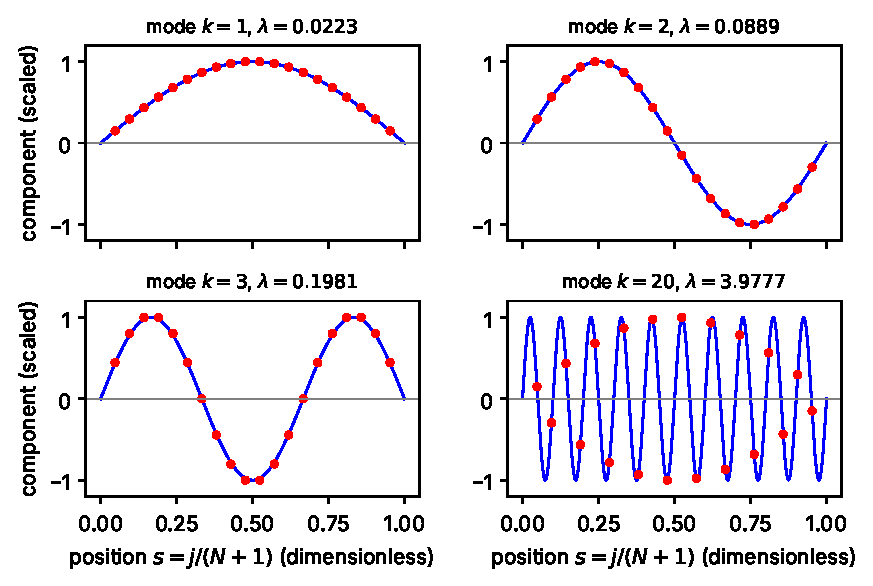
\includegraphics[width=0.85\linewidth]{figs/eigen_modes.pdf}
\caption{Eigenvectors of the $20\times20$ second-difference matrix $D_{20}$ computed numerically (dots), against the sine curves $\sin(k\pi s)$ (lines), with $s=j/21$ the position along the chain. Modes $k=1,2,3$ look like the first three harmonics of a string; the top mode $k=20$ alternates in sign from point to point and is a poor imitation of any smooth wave. Components are dimensionless.}
\label{fig:eigen-modes}
\end{figure}

\begin{checkpoint}
In Eq.~\eqref{eq:eigen-DN-eig}, why is $k=N+1$ not allowed?
\end{checkpoint}
\checkanswer{For $k=N+1$ the components are $\sin(jk\pi/(N+1))=\sin(j\pi)=0$ for every $j$, so the ``eigenvector'' is the zero vector, which is excluded by definition.}

\begin{keyideas}
\item Symmetric tridiagonal matrices need only $2N-1$ stored numbers.
\item If all off-diagonal entries are nonzero, every eigenvalue is simple, so eigenvalues can be numbered unambiguously in increasing order.
\item The second-difference matrix $D_N$ has eigenvalues $4\sin^2(k\pi/2(N+1))$ and sampled-sine eigenvectors, Eq.~\eqref{eq:eigen-DN-eig}; mode $k$ has $k-1$ sign changes.
\end{keyideas}

%==========================================================
\section{The second derivative as a matrix}\label{sec:eigen-second-derivative}

Recall from Chapter~\ref{ch:linear-algebra} that a function $f(x)$ on an interval can be represented by its values on a grid. Here we use the grid the paper uses. Divide $[-L,L]$ into $N+1$ equal steps of width
\begin{equation}
h=\frac{2L}{N+1},
\label{eq:eigen-h}
\end{equation}
and keep the $N$ \emph{interior} points
\begin{equation}
x_j=-L+jh,\qquad j=1,2,\dots,N.
\label{eq:eigen-grid}
\end{equation}
The endpoints $x_0=-L$ and $x_{N+1}=L$ are the walls. Write $f_j=f(x_j)$.

\paragraph{The second difference.} Expand $f$ about $x_j$ in a Taylor series (first-year calculus), assuming $f$ has at least six continuous derivatives. We use big-O notation: $\order(h^5)$, read ``order $h^5$'', stands for a quantity whose size is at most a fixed constant times $\abs{h}^5$ for all sufficiently small $h$. (Similarly, an algorithm whose cost is $\order(n^3)$ needs at most a fixed constant times $n^3$ operations for large $n$.) The expansions are:
\begin{align}
f(x_j+h)&=f_j+hf'_j+\tfrac{h^2}{2}f''_j+\tfrac{h^3}{6}f'''_j+\tfrac{h^4}{24}f''''_j+\order(h^5),\\
f(x_j-h)&=f_j-hf'_j+\tfrac{h^2}{2}f''_j-\tfrac{h^3}{6}f'''_j+\tfrac{h^4}{24}f''''_j+\order(h^5).
\end{align}
Adding the two lines, the odd powers of $h$ cancel:
\begin{equation}
f_{j+1}+f_{j-1}=2f_j+h^2f''_j+\tfrac{h^4}{12}f''''_j+\order(h^6),
\end{equation}
where the remainder is $\order(h^6)$ because the $h^5$ terms are odd in $h$ and cancel as well. Subtract $2f_j$ and divide by $h^2$:
\begin{equation}
\frac{f_{j+1}-2f_j+f_{j-1}}{h^2}=f''_j+\frac{h^2}{12}f''''_j+\order(h^4).
\label{eq:eigen-second-diff}
\end{equation}
So the ``second difference'' on the left approximates $f''(x_j)$ with an error of order $h^2$. Chapter~\ref{ch:finite-differences} studies this error carefully; here we need only the structure.

\paragraph{The matrix.} Multiply Eq.~\eqref{eq:eigen-second-diff} by $-1$ and impose the wall conditions $f_0=f_{N+1}=0$ (the function vanishes at the walls, like a string tied down there). Then the list of values $-f''(x_j)$ is approximated by
\begin{equation}
-f''(x_j)\approx\frac{1}{h^2}\bigl(-f_{j-1}+2f_j-f_{j+1}\bigr)=\frac{1}{h^2}(D_Nf)_j,
\end{equation}
with $D_N$ of Eq.~\eqref{eq:eigen-DN}. In the first row, $f_0=0$ removes the term $-f_0$; in the last row, $f_{N+1}=0$ removes $-f_{N+1}$. So the operator ``take minus the second derivative of a function vanishing at $\pm L$'' becomes the matrix $D_N/h^2$.

\paragraph{Adding a potential.} In quantum mechanics (Chapter~\ref{ch:schrodinger}) the energy operator, the Hamiltonian, in the units $\hbar=2m=1$ that the paper uses, is
\begin{equation}
H=-\frac{d^2}{dx^2}+V(x).
\end{equation}
The potential $V(x)$ multiplies the wavefunction point by point, which on the grid is the diagonal matrix $\operatorname{diag}(V(x_1),\dots,V(x_N))$. Adding,
\begin{equation}
\boxed{H_{jj}=\frac{2}{h^2}+V(x_j),\qquad H_{j,j\pm1}=-\frac{1}{h^2},\qquad\text{all other entries }0.}
\label{eq:eigen-Hmatrix}
\end{equation}
This is a real symmetric tridiagonal matrix with every off-diagonal entry equal to $-1/h^2\ne0$. Everything proved so far applies: its eigenvalues are real (Theorem 1), distinct (nondegeneracy theorem of \cref{sec:eigen-tridiagonal}), and its eigenvectors form an orthonormal basis of real vectors (spectral theorem). The eigenvalues approximate the energy levels; the eigenvectors are the wavefunctions sampled on the grid.

\paragraph{The empty box exactly.} With $V=0$ the eigenvalues of $D_N/h^2$ follow from Eq.~\eqref{eq:eigen-DN-eig} by dividing by $h^2$. Since $N+1=2L/h$ by Eq.~\eqref{eq:eigen-h}, the angle $k\pi/(2(N+1))$ equals $k\pi h/(4L)$, and
\begin{equation}
\lambda_k^{\rm disc}=\frac{4}{h^2}\sin^2\frac{k\pi h}{4L},\qquad
(v_k)_j=\sin\frac{jk\pi}{N+1}=\sin\frac{k\pi(x_j+L)}{2L}.
\label{eq:eigen-box-disc}
\end{equation}
For the second form of the eigenvector we used $x_j+L=jh=2Lj/(N+1)$, so $jk\pi/(N+1)=k\pi(x_j+L)/(2L)$. We will see in the next section that $\sin(k\pi(x+L)/2L)$ is exactly the $k$-th eigenfunction of the continuous problem. So the discrete eigenvectors are the exact continuous eigenfunctions sampled at the grid points, and only the eigenvalues carry a discretization error.

\begin{keyideas}
\item The second difference $(f_{j+1}-2f_j+f_{j-1})/h^2$ approximates $f''$ with error $\order(h^2)$, Eq.~\eqref{eq:eigen-second-diff}.
\item With walls at $\pm L$, $-d^2/dx^2$ becomes $D_N/h^2$, and $H=-d^2/dx^2+V$ becomes the symmetric tridiagonal matrix of Eq.~\eqref{eq:eigen-Hmatrix}.
\item For the empty box the discrete eigenvalues are $(4/h^2)\sin^2(k\pi h/4L)$ and the eigenvectors are sampled sines, Eq.~\eqref{eq:eigen-box-disc}.
\end{keyideas}

%==========================================================
\section{Eigenvalue problems for differential operators}\label{sec:eigen-ode}

Now forget the grid and ask the continuous question. Which functions $y(x)$ on $[-L,L]$, vanishing at both ends, satisfy
\begin{equation}
-y''(x)=\lambda\,y(x),\qquad y(-L)=y(L)=0,
\label{eq:eigen-string}
\end{equation}
for some number $\lambda$, with $y$ not identically zero? This is an eigenvalue problem in which the ``matrix'' is the operator $-d^2/dx^2$ and the ``vectors'' are functions. It is also the equation of a standing wave on a string of length $2L$ fixed at both ends: for a shape $y(x)\cos(\omega t)$ the wave equation reduces to Eq.~\eqref{eq:eigen-string} with $\lambda=\omega^2/c_{\rm w}^2$, where $\omega$ is the angular frequency of the standing wave and $c_{\rm w}$ the wave speed \cite{hrw}. And in Chapter~\ref{ch:bound-states} it will be the Schr\"odinger equation for a particle in a box, with $\lambda$ the energy.

\paragraph{The eigenvalues are real and non-negative.} Before solving, we show that $\lambda$ must be real. Allow $y$ and $\lambda$ to be complex for the moment. Multiply both sides of $-y''=\lambda y$ by $y^*$, the complex conjugate of $y$, and integrate over $[-L,L]$:
\begin{align}
\lambda\int_{-L}^L\abs{y}^2\,\dd x&=-\int_{-L}^Ly^*y''\,\dd x\\
&=\bigl[-y^*y'\bigr]_{-L}^{L}+\int_{-L}^L(y^*)'\,y'\,\dd x\quad\text{(parts: }u=y^*,\ \dd v=-y''\dd x)\\
&=\int_{-L}^L\abs{y'}^2\,\dd x.\quad\text{(}y(\pm L)=0\text{ and }(y^*)'=(y')^*)
\end{align}
Both integrals are real and non-negative. Also $\int\abs{y}^2\dd x>0$, because $y$ is not identically zero. So $\lambda=\int\abs{y'}^2\dd x\big/\int\abs{y}^2\dd x$ is real and $\lambda\ge0$. This is the continuous analogue of Eq.~\eqref{eq:eigen-rayleigh-eig}.

\paragraph{Solving it completely.} Knowing that $\lambda$ is real, we still consider all three possible signs of $\lambda$ in turn, which also confirms that $\lambda\le0$ gives nothing.

\emph{Case $\lambda=0$.} Then $y''=0$, so $y=a+bx$. The conditions give $a-bL=0$ and $a+bL=0$; adding, $2a=0$, so $a=0$; then $bL=0$, so $b=0$. Only $y\equiv0$: no eigenvalue.

\emph{Case $\lambda<0$.} Write $\lambda=-\kappa^2$ with $\kappa>0$. Then $y''=\kappa^2y$, with general solution $y=ae^{\kappa x}+be^{-\kappa x}$ (check by differentiating twice). The conditions are $ae^{-\kappa L}+be^{\kappa L}=0$ and $ae^{\kappa L}+be^{-\kappa L}=0$. From the first, $a=-be^{2\kappa L}$. Substituting into the second, $-be^{3\kappa L}+be^{-\kappa L}=b(e^{-\kappa L}-e^{3\kappa L})=0$. Since $\kappa L>0$, $e^{3\kappa L}>e^{-\kappa L}$, so $b=0$ and then $a=0$. No eigenvalue.

\emph{Case $\lambda>0$.} Write $\lambda=q^2$ with $q>0$. Then $y''=-q^2y$, which is the simple-harmonic-motion equation with $x$ in place of time, with general solution $y=a\cos(qx)+b\sin(qx)$. The conditions, using $\cos$ even and $\sin$ odd, are
\begin{align}
y(L)&=a\cos(qL)+b\sin(qL)=0,\\
y(-L)&=a\cos(qL)-b\sin(qL)=0.
\end{align}
Adding gives $2a\cos(qL)=0$; subtracting gives $2b\sin(qL)=0$. For a nonzero solution, either $a\ne0$ and $\cos(qL)=0$, i.e.\ $qL=\pi/2,3\pi/2,\dots$ (odd multiples of $\pi/2$), with $b=0$ because $\sin(qL)=\pm1\ne0$ there; or $b\ne0$ and $\sin(qL)=0$, i.e.\ $qL=\pi,2\pi,\dots$ (even multiples of $\pi/2$), with $a=0$. Both families together are $qL=k\pi/2$ with $k=1,2,3,\dots$. Hence
\begin{equation}
\boxed{\lambda_k=\left(\frac{k\pi}{2L}\right)^2,\qquad y_k(x)=\sin\frac{k\pi(x+L)}{2L},\qquad k=1,2,3,\dots}
\label{eq:eigen-string-sol}
\end{equation}
The single formula for $y_k$ covers both families: $\sin(k\pi x/(2L)+k\pi/2)$ equals $\pm\cos(k\pi x/2L)$ for odd $k$ and $\pm\sin(k\pi x/2L)$ for even $k$. In the language of the string, the wavelength of mode $k$ is $2\cdot2L/k$, and the wavenumber $q=2\pi/\text{wavelength}=k\pi/(2L)$, the familiar harmonics \cite{hrw}.

Unlike a matrix, the operator has infinitely many eigenvalues, growing without bound like $k^2$. The $N\times N$ matrix $D_N/h^2$ can only capture the first $N$ of them, and (as we will compute) only the first part of those accurately.

\paragraph{The operator is symmetric.} Why are the eigenvalues real and the eigenfunctions orthogonal, exactly as for symmetric matrices? Because $-d^2/dx^2$ with these boundary conditions has the continuous version of the symmetry property. Recall from Chapter~\ref{ch:linear-algebra} that for real functions the inner product is $\int_{-L}^Lf(x)g(x)\,\dd x$. Let $f,g$ be twice differentiable with $f(\pm L)=g(\pm L)=0$. Integrate by parts:
\begin{align}
\int_{-L}^Lf\,(-g'')\,\dd x&=\bigl[-fg'\bigr]_{-L}^{L}+\int_{-L}^Lf'g'\,\dd x\quad\text{(parts: }u=f,\ \dd v=-g''\dd x)\\
&=\int_{-L}^Lf'g'\,\dd x\quad\text{(}f(\pm L)=0)\\
&=\bigl[f'g\bigr]_{-L}^{L}-\int_{-L}^Lf''g\,\dd x\quad\text{(parts: }u=g,\ \dd v=f'\dd x)\\
&=\int_{-L}^L(-f'')\,g\,\dd x.\quad\text{(}g(\pm L)=0)
\label{eq:eigen-parts}
\end{align}
This is the function version of $u^\top Av=(Au)^\top v$. Adding a real potential keeps the property, since $\int f\,(Vg)\,\dd x=\int(Vf)\,g\,\dd x$ trivially. Now repeat the proof of Theorem 2 with integrals: if $-y_k''=\lambda_ky_k$ and $-y_l''=\lambda_ly_l$, Eq.~\eqref{eq:eigen-parts} with $f=y_k$, $g=y_l$ gives $\lambda_l\int y_ky_l\,\dd x=\lambda_k\int y_ky_l\,\dd x$, so $\int y_ky_l\,\dd x=0$ when $\lambda_k\ne\lambda_l$. Readers who have studied Fourier series (Chapter~\ref{ch:fourier-series}) will recognize this as the orthogonality of the sines of Eq.~\eqref{eq:eigen-string-sol}. Here it has been derived without evaluating any trigonometric integral.

\begin{beyond}
\textbf{Taken on trust: ``self-adjoint'' in infinite dimensions.} For operators on infinitely many dimensions, such as $-d^2/dx^2$ acting on functions, the property of Eq.~\eqref{eq:eigen-parts} (called ``symmetric'' or ``Hermitian'') is not by itself enough to guarantee all the conclusions of the spectral theorem. One needs a stronger condition, \emph{self-adjointness}, which also specifies precisely which functions the operator acts on (its ``domain''; here, the boundary conditions). For a Schr\"odinger operator on a finite interval with walls, the two notions coincide, and the conclusions (real eigenvalues, orthonormal eigenfunctions forming a basis) hold. The precise definitions and proofs belong to functional analysis and are beyond this book; a physicist's account is in \cite{griffiths}. When the paper says ``self-adjoint operator'', you can read ``the infinite-dimensional analogue of a Hermitian matrix, whose eigenvalues are therefore real''.
\end{beyond}

\begin{sample}{The box of RE3: continuum versus grid}
Take the box of the running example RE3, $L=44.883$, which is the half-width the paper uses at scale 1. (a) Find the first three eigenvalues of Eq.~\eqref{eq:eigen-string}. (b) For the grid the paper uses at scale 1, $N=6000$, compare the exact $\lambda_{500}$ with the matrix eigenvalue of $D_N/h^2$, and express the difference in units of the local spacing between exact eigenvalues.

\textbf{Step 1: lowest eigenvalues.} $\pi/(2L)=\pi/89.766=0.0349976$, so $\lambda_1=(\pi/2L)^2=1.2248\times10^{-3}$, $\lambda_2=4\lambda_1=4.8993\times10^{-3}$, $\lambda_3=9\lambda_1=1.10235\times10^{-2}$.

\textbf{Step 2: grid spacing.} $h=2L/(N+1)=89.766/6001=0.014958$.

\textbf{Step 3: exact $\lambda_{500}$.} $500\pi/(2L)=17.4988$, so $\lambda_{500}=(17.4988)^2=306.208$.

\textbf{Step 4: matrix eigenvalue.} By Eq.~\eqref{eq:eigen-box-disc} with the angle $500\pi h/(4L)=500\pi/(2\cdot6001)=0.130878$:
\[
\lambda_{500}^{\rm disc}=\frac{4}{h^2}\sin^2(0.130878)=304.463.
\]
A direct numerical eigensolve of the $6000\times6000$ matrix (Listing in \cref{sec:eigen-numerics}) gives the same number.

\textbf{Step 5: difference and spacing.} $306.208-304.463=1.744$. The spacing of exact eigenvalues near $k=500$ is $\lambda_{501}-\lambda_{500}=(\pi/2L)^2(501^2-500^2)=(\pi/2L)^2\cdot1001=1.2261$. The ratio is $1.744/1.2261=1.42$.

\[
\boxed{\lambda_{1,2,3}=1.2248\times10^{-3},\ 4.8993\times10^{-3},\ 1.10235\times10^{-2};\quad \lambda_{500}=306.208\ \text{vs}\ 304.463,\ \text{off by }1.42\ \text{spacings}.}
\]
Even with 6000 grid points, level 500 of the matrix is more than a full level spacing below the true level. This is a warning that you will hear again: the paper (Sec.~II~C, paragraph ``No leakage through the bias correction'') reports that for its potential at levels 401--500 on the working grid the finite-difference error ``reaches two mean spacings''. Chapter~\ref{ch:finite-differences} explains how the paper removes it.
\end{sample}

\Cref{tab:eigen-box} and \cref{fig:eigen-spectrum} show the pattern. Expanding $\sin y=y-y^3/6+\dots$ gives $\sin^2y=y^2-y^4/3+\dots$, so with $y=k\pi h/4L$,
\begin{equation}
\lambda_k^{\rm disc}=\left(\frac{k\pi}{2L}\right)^2\left[1-\frac13\left(\frac{k\pi h}{4L}\right)^2+\dots\right]:
\end{equation}
the relative error grows like $k^2h^2$. This agrees with Eq.~\eqref{eq:eigen-second-diff}: for $y=\sin(qx+\dots)$, $y''''=q^4y$, so the error term $\tfrac{h^2}{12}y''''$ changes $q^2$ by $-\tfrac{h^2}{12}q^4$, a relative change $h^2q^2/12=k^2\pi^2h^2/(48L^2)$, which is the same as $\tfrac13(k\pi h/4L)^2$.

\begin{table}[htbp]\centering
\caption{Eigenvalues of $-d^2/dx^2$ on $[-L,L]$ with $L=44.883$: exact $(k\pi/2L)^2$ versus the $N=6000$ matrix $D_N/h^2$, Eq.~\eqref{eq:eigen-box-disc}. Relative error $=1-\lambda^{\rm disc}_k/\lambda_k$.}
\label{tab:eigen-box}
\begin{tabular}{rccc}
\toprule
$k$ & exact & matrix & relative error\\
\midrule
1 & $1.2248\times10^{-3}$ & $1.2248\times10^{-3}$ & $2.28\times10^{-8}$\\
10 & $0.12248$ & $0.12248$ & $2.28\times10^{-6}$\\
100 & $12.2483$ & $12.2455$ & $2.28\times10^{-4}$\\
500 & $306.208$ & $304.463$ & $5.70\times10^{-3}$\\
\bottomrule
\end{tabular}
\end{table}

\begin{figure}[htbp]\centering
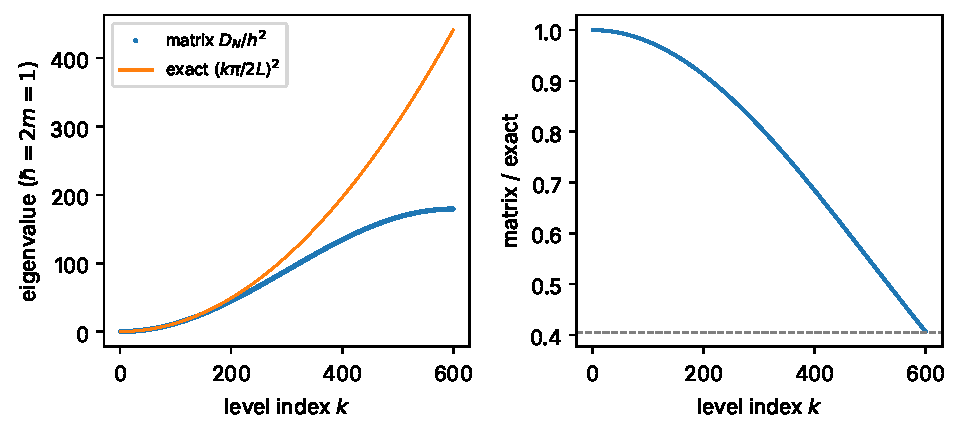
\includegraphics[width=0.85\linewidth]{figs/eigen_spectrum.pdf}
\caption{Left: all $N=600$ eigenvalues of the matrix $D_N/h^2$ for the box $[-L,L]$ with $L=44.883$ (dots) against the exact continuum eigenvalues $(k\pi/2L)^2$ (line); energies in units $\hbar=2m=1$. Right: their ratio, which is $1$ for low $k$ and falls to about $0.41$ at $k=N$. A coarse grid is used so that the deviation is visible; it is the same phenomenon as in \cref{tab:eigen-box}.}
\label{fig:eigen-spectrum}
\end{figure}

\begin{keyideas}
\item $-y''=\lambda y$ with $y(\pm L)=0$ has eigenvalues $(k\pi/2L)^2$ and eigenfunctions $\sin(k\pi(x+L)/2L)$, Eq.~\eqref{eq:eigen-string-sol}: the harmonics of a string.
\item With these boundary conditions $-d^2/dx^2+V$ is symmetric, Eq.~\eqref{eq:eigen-parts}, so its eigenvalues are real and its eigenfunctions orthogonal; ``self-adjoint'' is the precise infinite-dimensional notion.
\item The grid matrix reproduces low eigenvalues well, but the relative error grows like $k^2h^2$; at $N=6000$, level 500 of the empty box is off by about $1.4$ level spacings.
\end{keyideas}

%==========================================================
\section{Numerical eigensolvers}\label{sec:eigen-numerics}

For a $6000\times6000$ matrix no human will expand a determinant. Computers find eigenvalues by iterative algorithms, packaged in libraries that you can treat as black boxes, provided you know what goes in, what comes out, and roughly how long it takes.

\paragraph{Why iteration?} Finding eigenvalues of an $n\times n$ matrix is equivalent to finding the roots of a polynomial of degree $n$. For degree $5$ and higher there is no general formula built from arithmetic operations and roots (see the box below). So every eigenvalue algorithm for large matrices is iterative: it produces a sequence of better and better approximations and stops when the error is at the level of rounding.

\begin{beyond}
\textbf{Taken on trust: the Abel--Ruffini theorem.} There is no formula that expresses the roots of every polynomial of degree $5$ or higher in terms of its coefficients using only addition, subtraction, multiplication, division and $k$-th roots. The proof belongs to Galois theory and is found in standard texts on abstract algebra. Every polynomial with leading coefficient $1$ is, up to sign, the characteristic polynomial of some matrix (a so-called companion matrix), so no such formula can exist for the eigenvalues of general $n\times n$ matrices with $n\ge5$ either.
\end{beyond}

\paragraph{What LAPACK does.} LAPACK (Linear Algebra PACKage) is the standard, freely available library of linear algebra routines that numpy and scipy call internally. For a dense real symmetric or complex Hermitian matrix, its strategy has three stages \cite{trefethen}:
\begin{enumerate}
\item \emph{Reduce to tridiagonal form.} A sequence of carefully chosen unitary matrices $Q$ (Householder reflections) turns $A$ into $Q^\dagger AQ=T$, tridiagonal. A transformation of this form does not change eigenvalues (Problem~29 shows that $S^{-1}AS$ always has the same characteristic polynomial as $A$, and $Q^\dagger=Q^{-1}$). This stage costs about $\tfrac43n^3$ arithmetic operations \cite{trefethen}.
\item \emph{Solve the tridiagonal problem} by an iterative method (the QR iteration, divide-and-conquer, or bisection; see below).
\item \emph{Transform the eigenvectors back} by multiplying by $Q$.
\end{enumerate}
For a dense non-Hermitian matrix (such as the complex matrix $H+iA$ of the paper's Sec.~II~E), LAPACK first reduces to a form with zeros below the first sub-diagonal (``Hessenberg form'') and then applies the QR iteration; the cost again grows like $n^3$, with a larger constant. Because of stage 1, the cost of a dense eigensolve is $\order(n^3)$: doubling $n$ multiplies the work by about $8$.

If your matrix is \emph{already} tridiagonal, as Eq.~\eqref{eq:eigen-Hmatrix} is, you skip stage 1 entirely and the cost drops to $\order(n^2)$ for all eigenvalues, and less if you want only some of them. To see why, look at bisection.

\paragraph{Counting eigenvalues below a number: the Sturm count.} For the symmetric tridiagonal matrix \eqref{eq:eigen-tridiag} and a trial number $x$, compute the sequence
\begin{equation}
q_1=d_1-x,\qquad q_j=d_j-x-\frac{b_{j-1}^2}{q_{j-1}},\quad j=2,\dots,N.
\label{eq:eigen-sturm}
\end{equation}
These $q_j$ are the pivots that Gaussian elimination (Chapter~\ref{ch:linear-algebra}) produces when it reduces $T-xI$ to triangular form without swapping rows: eliminating the entry $b_{j-1}$ below the pivot $q_{j-1}$ subtracts $(b_{j-1}/q_{j-1})\times$ row $j-1$ from row $j$, which changes the diagonal entry $d_j-x$ into $d_j-x-b_{j-1}^2/q_{j-1}$. Their product is therefore $\det(T-xI)$, which equals $\prod_k(\lambda_k-x)$ by the factorization of the characteristic polynomial in \cref{sec:eigen-charpoly}.

\begin{beyond}
\textbf{Taken on trust: Sturm count (Sylvester's law of inertia).} If no $q_j$ is exactly zero, the number of negative values among $q_1,\dots,q_N$ equals the number of eigenvalues of $T$ that are less than $x$. The product formula above shows only that the two counts have the same parity (both even or both odd); the full statement is a consequence of Sylvester's law of inertia, proved in \cite{trefethen} and \cite{nr}.
\end{beyond}

Each Sturm count costs $\order(N)$ operations. To pin down eigenvalue number $k$, start with an interval known to contain it and \emph{bisect} it, that is, keep halving it and retain the half that contains the target: at the midpoint, the count tells you whether $\lambda_k$ lies to the left or right. Each step halves the interval, so reaching double precision from a reasonable starting interval takes a few dozen steps. All $N$ eigenvalues then cost $N\times(\text{a few dozen})\times\order(N)=\order(N^2)$. The eigenvectors can be obtained afterwards by solving a few tridiagonal linear systems per eigenvalue (``inverse iteration''), each $\order(N)$. The same count also answers the question ``how many levels lie below $E$?'' in $\order(N)$ operations, which is one standard way (bisection with Sturm counts) for a solver to return ``all eigenvalues in a range''.

\begin{pycode}
import numpy as np

def sturm_count(d, b, x):
    """Number of eigenvalues < x of the symmetric tridiagonal
    matrix with diagonal d (length N) and off-diagonal b (N-1)."""
    count = 0
    q = d[0] - x
    for j in range(len(d)):
        if j > 0:
            q = d[j] - x - b[j-1]**2 / q
        if q == 0.0:          # exact zero pivot: nudge it
            q = -1e-300
        if q < 0:
            count += 1
    return count

d = np.array([2.0, 2.0, 2.0]); b = np.array([-1.0, -1.0])
print(sturm_count(d, b, 2.5), sturm_count(d, b, 0.6))   # 2 1
\end{pycode}

\begin{sample}{Counting levels by hand}
Use the Sturm count \eqref{eq:eigen-sturm} to find how many eigenvalues of $D_3$ lie below $x=2.5$ and below $x=0.6$, and compare with the exact eigenvalues $0.585786,\ 2,\ 3.414214$.

\textbf{Step 1: $x=2.5$.} $d_j-x=-0.5$, $b_j^2=1$. Then $q_1=-0.5$; $q_2=-0.5-1/(-0.5)=-0.5+2=1.5$; $q_3=-0.5-1/1.5=-1.16667$. Negative pivots: $q_1,q_3$, two of them.

\textbf{Step 2: compare.} The eigenvalues below $2.5$ are $0.585786$ and $2$: two. Agreement.

\textbf{Step 3: $x=0.6$.} $d_j-x=1.4$. Then $q_1=1.4$; $q_2=1.4-1/1.4=0.685714$; $q_3=1.4-1/0.685714=1.4-1.458333=-0.058333$. One negative pivot.

\textbf{Step 4: compare.} Only $0.585786<0.6$: one. Agreement, and the small size of $q_3$ reflects how close $0.6$ is to an eigenvalue.

\[
\boxed{\text{count}(2.5)=2,\qquad\text{count}(0.6)=1.}
\]
\end{sample}

\paragraph{The tools you will actually call.} \Cref{tab:eigen-solvers} lists the functions used in this book. All of them call LAPACK.

\begin{table}[htbp]\centering
\caption{Eigensolvers in numpy and scipy.}
\label{tab:eigen-solvers}
\begin{tabular}{lll}
\toprule
function & for & returns\\
\midrule
\texttt{np.linalg.eigh(A)} & dense Hermitian/symmetric & real eigenvalues, ascending; orthonormal vectors\\
\texttt{np.linalg.eig(A)} & any dense square matrix & complex eigenvalues, \emph{no particular order}\\
\texttt{scipy.linalg.eigh\_tridiagonal(d, e, ...)} & real symmetric tridiagonal & ascending eigenvalues, optionally a subset\\
\bottomrule
\end{tabular}
\end{table}

For \texttt{eigh\_tridiagonal}, \texttt{d} is the diagonal and \texttt{e} the off-diagonal. The option \texttt{select='i', select\_range=(0, k-1)} returns the lowest $k$ eigenpairs (indices start at 0 in Python); \texttt{select='v', select\_range=(lo, hi)} returns those with $\text{lo}<\lambda\le\text{hi}$. The eigenvectors are returned as the columns of a matrix.

\begin{pycode}
import numpy as np
from scipy.linalg import eigh_tridiagonal

L, N = 44.883, 6000                     # RE3 box, paper's scale-1 grid
h = 2*L/(N + 1)
V = np.zeros(N)                         # empty box; put V(x_j) here
d = 2/h**2 + V                          # diagonal, Eq. (eigen-Hmatrix)
e = -np.ones(N - 1)/h**2                # off-diagonal
E, psi = eigh_tridiagonal(d, e, select='i', select_range=(0, 499))
psi = psi/np.sqrt(h)                    # now sum(psi**2)*h = 1
k = np.arange(1, 501)
exact = (k*np.pi/(2*L))**2
print(E[499], exact[499])               # 304.463...  306.208...
\end{pycode}

\begin{pitfall}
\textbf{Normalization conventions.} Solvers return eigenvectors with $\sum_j v_j^2=1$. A wavefunction sampled on a grid should instead satisfy $\sum_j\psi_j^2h\approx\int\psi^2\dd x=1$. The two differ by the factor $1/\sqrt h$, as in the listing above. Forgetting the rescaling makes every such integral, computed as $\sum_jv_j^2\phi_k(x_j)h$, too small by a factor $h$. Rescaling but forgetting the $h$ in the sum makes it too large by a factor $1/h$.
\end{pitfall}

\begin{pitfall}
\textbf{Signs and order.} The sign (or complex phase) of each returned eigenvector is arbitrary and may change between runs or library versions; never compare eigenvectors without fixing it or using quantities like $\abs{u^\dagger w}^2$ that do not depend on it. \texttt{np.linalg.eig} returns eigenvalues in no particular order; always sort, or match (\cref{sec:eigen-matching}). Finally, do not use \texttt{eig} on a symmetric matrix: rounding can produce tiny spurious imaginary parts; use \texttt{eigh}.
\end{pitfall}

\paragraph{How accurate are computed eigenvalues?} The computer works in floating-point arithmetic with machine epsilon $\epsilon\approx2.2\times10^{-16}$ in double precision. This is the relative gap between neighboring representable numbers near $1$, so each arithmetic operation can introduce a relative rounding error of about this size.

\begin{beyond}
\textbf{Taken on trust: stability of Hermitian eigenvalues.} The LAPACK symmetric eigensolvers are \emph{backward stable}: the eigenvalues they return are the exact eigenvalues of a slightly perturbed matrix $A+E$ with the size of $E$ about $\epsilon$ times the size of $A$. For Hermitian matrices, Weyl's inequality guarantees that perturbing $A$ by $E$ moves each eigenvalue by at most the size (largest singular value, Chapter~\ref{ch:least-squares}) of $E$. Together: computed eigenvalues of a Hermitian matrix are accurate to about $\epsilon$ times the largest $\abs{\lambda}$. Proofs in \cite{trefethen}. Non-Hermitian matrices enjoy no such guarantee; their eigenvalues can be far more sensitive.
\end{beyond}

For the matrix of the listing, the largest eigenvalue is close to $4/h^2\approx1.79\times10^4$. Adding the Wu--Sprung potential, which reaches $1000$ at scale 1, raises it by at most $1000$. So rounding errors in the eigenvalues are a few times $10^{-12}$: utterly negligible against the $\order(1)$ discretization errors of \cref{tab:eigen-box}. The numerical eigensolver is not the weak link; the grid is.

\Cref{fig:eigen-wavefunctions} shows what the same code produces when $V$ is the Wu--Sprung potential of the paper's Eq.~(2), which you will study in Chapter~\ref{ch:wu-sprung}.

\begin{figure}[htbp]\centering
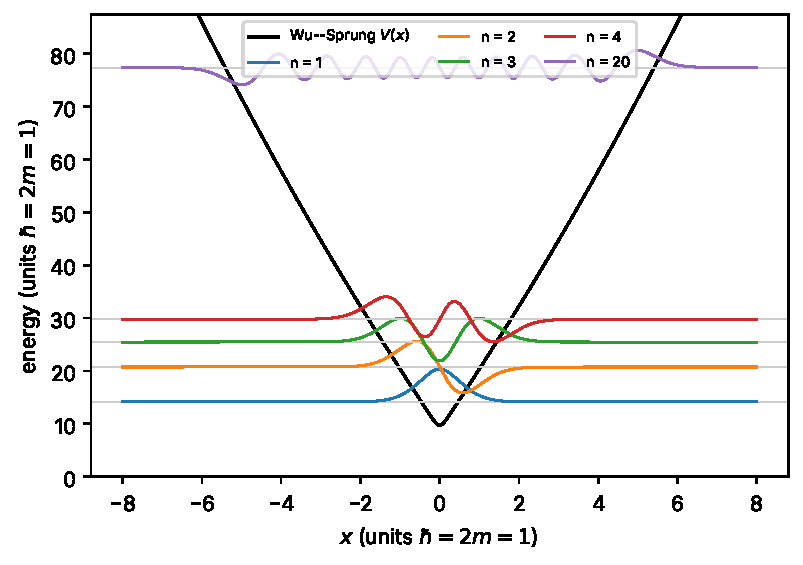
\includegraphics[width=0.85\linewidth]{figs/eigen_wavefunctions.pdf}
\caption{Eigenvectors of the tridiagonal matrix \eqref{eq:eigen-Hmatrix} with $V$ the Wu--Sprung potential (paper Eq.~(2)) on $[-L,L]$, $L=44.883$, $N=4000$. Each eigenvector (normalized so that $\sum\psi^2h=1$, then magnified for visibility) is drawn at the height of its eigenvalue; only $\abs{x}\le8$ is shown. Levels $n=1,2,3,4$ and $n=20$ are shown. Each state oscillates where $E_n>V$ and decays beyond its classical turning points; state $n$ has $n-1$ sign changes; states alternate between even and odd because $V$ is even. Units $\hbar=2m=1$.}
\label{fig:eigen-wavefunctions}
\end{figure}

\begin{checkpoint}
Roughly how many times more arithmetic does a dense symmetric eigensolve of a $6000\times6000$ matrix need than computing all eigenvalues of a $6000\times6000$ tridiagonal matrix, if the costs are $n^3$ and $n^2$ up to similar constants?
\end{checkpoint}
\checkanswer{The ratio is $n^3/n^2=n=6000$. Using the tridiagonal structure saves a factor of thousands.}

\begin{keyideas}
\item Eigenvalues of large matrices are found iteratively by library routines (LAPACK) that you may treat as black boxes.
\item Dense Hermitian or non-Hermitian eigensolves cost $\order(n^3)$; symmetric tridiagonal ones cost $\order(n^2)$ for all eigenvalues.
\item The Sturm count, Eq.~\eqref{eq:eigen-sturm}, counts eigenvalues below $x$ in $\order(N)$ operations and powers bisection and ``eigenvalues in a range''.
\item Mind conventions: eigenvectors come with $\sum v^2=1$ (rescale by $1/\sqrt h$ for wavefunctions), arbitrary signs, and (for \texttt{eig}) no ordering.
\item Computed Hermitian eigenvalues are accurate to about $\epsilon$ times the largest eigenvalue.
\end{keyideas}

%==========================================================
\section{Ordering eigenvalues and matching eigenvectors}\label{sec:eigen-matching}

In the paper, ``level $n$'' of a fitted potential is compared with ``zero $n$''. That requires a labelling of eigenvalues by an index $n$ that means the same thing before and after the potential is changed. For Hermitian matrices there is a natural labelling; for non-Hermitian ones there is not, and one must match eigenvectors instead.

\paragraph{Hermitian case: order by size.} Real eigenvalues can be sorted, $\lambda_1<\lambda_2<\dots$. For the tridiagonal Hamiltonian \eqref{eq:eigen-Hmatrix} they are all distinct (\cref{sec:eigen-tridiagonal}) for \emph{every} potential, so the $n$-th eigenvalue is well defined. Even more is true: as you change $V$ smoothly, the eigenvalues move continuously. This follows from Weyl's inequality (taken on trust in the box of \cref{sec:eigen-numerics}): changing $V$ by at most $\delta$ at every grid point adds a diagonal matrix whose largest singular value is at most $\delta$, so each eigenvalue moves by at most $\delta$. Two of them can never meet, because meeting would be a degeneracy. So the $n$-th level stays the $n$-th level; levels cannot overtake one another.

But ``the $n$-th level'' and ``the state that looks like the original state $n$'' need not be the same thing. Consider
\begin{equation}
H(\varepsilon)=\begin{pmatrix}\varepsilon&g\\g&-\varepsilon\end{pmatrix},\qquad g>0\ \text{fixed},
\label{eq:eigen-avoided}
\end{equation}
as the parameter $\varepsilon$ is swept from negative to positive. Here $\operatorname{tr}H=0$ and $\det H=-\varepsilon^2-g^2$, so Eq.~\eqref{eq:eigen-quadratic} gives $\lambda_\pm=\pm\sqrt{\varepsilon^2+g^2}$. Without the coupling ($g=0$) the two levels $\pm\varepsilon$ would cross at $\varepsilon=0$; with it, they come no closer than $2g$. This is an \emph{avoided crossing} (\cref{fig:eigen-avoided}, left). Far to the left ($\varepsilon\ll-g$) the lower eigenvector is almost $e_1=(1,0)^\top$; far to the right it is almost $e_2$ (Problem~27 gives the exact formula). By ordering, the ``lower level'' is followed smoothly; by character, the states have exchanged identities. Which labelling is right depends on what question you ask. The paper's operator fits use ordering, which is natural for one-dimensional Hamiltonians (Chapter~\ref{ch:bound-states}: the $n$-th level always has $n-1$ nodes).

\begin{figure}[htbp]\centering
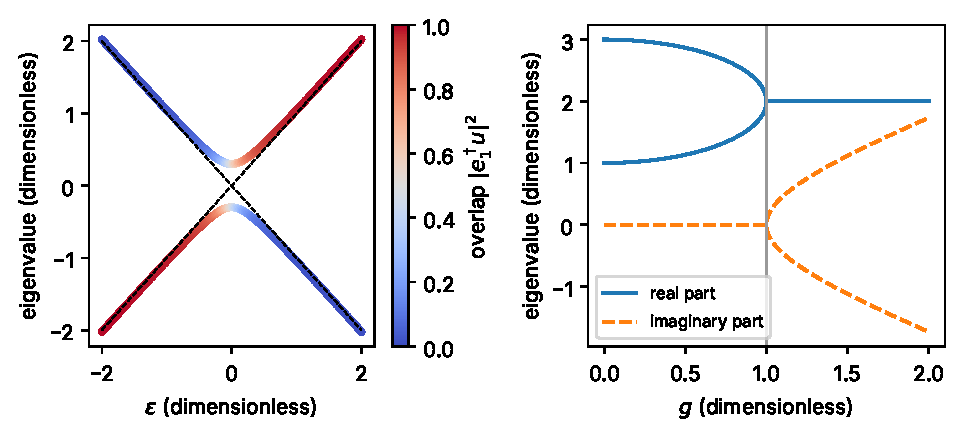
\includegraphics[width=0.85\linewidth]{figs/eigen_avoided.pdf}
\caption{Left: eigenvalues of the Hermitian matrix \eqref{eq:eigen-avoided} with $g=0.3$ versus $\varepsilon$; color gives the overlap $\abs{e_1^\dagger u}^2$ of each eigenvector with $e_1$. The levels avoid each other and exchange character. Dashed: the uncoupled levels $\pm\varepsilon$. Right: the non-Hermitian matrix $\begin{pmatrix}1&ig\\ig&3\end{pmatrix}$ versus $g$: real parts (solid) attract and merge at $g=1$, after which the eigenvalues become a complex-conjugate pair (imaginary parts, dashed). All quantities dimensionless.}
\label{fig:eigen-avoided}
\end{figure}

\paragraph{Non-Hermitian case: no natural order.} If eigenvalues are complex, ``sort by size'' has no meaning: complex numbers have no natural order. Sorting by real part is a common guess, but it can mislabel states, for example when two eigenvalues have equal real parts (right panel of \cref{fig:eigen-avoided}, $g>1$), or when a large imaginary part accompanies a small real shift. The robust approach is to compare \emph{eigenvectors}.

\paragraph{Matching by overlap.} Let $e_1,\dots,e_n$ be an orthonormal reference basis, typically the eigenvectors of the unperturbed Hermitian Hamiltonian, and let $w_1,\dots,w_n$ be the eigenvectors of the new (perturbed) matrix. Define the \emph{overlap matrix}
\begin{equation}
O_{km}=\frac{\abs{e_k^\dagger w_m}^2}{w_m^\dagger w_m}.
\label{eq:eigen-overlap}
\end{equation}
It does not depend on the arbitrary length or phase of $w_m$ (multiplying $w_m$ by $a$ multiplies the numerator and denominator by $\abs a^2$). Since the $e_k$ form an orthonormal basis, expanding $w_m=\sum_k(e_k^\dagger w_m)e_k$ gives $w_m^\dagger w_m=\sum_k\abs{e_k^\dagger w_m}^2$, so every \emph{column} sums to one:
\begin{equation}
\sum_{k=1}^nO_{km}=1.
\label{eq:eigen-colsum}
\end{equation}
$O_{km}$ is the fraction of $w_m$ that lies along reference state $e_k$. The matching rule: assign each new eigenvector $w_m$ to the reference state $k$ with the largest $O_{km}$, and call the matching \emph{one-to-one} if no two new eigenvectors are assigned to the same reference state.

\textbf{When is the matching guaranteed one-to-one? (proved)} If an entry $O_{km}>\tfrac12$, it is the largest in its column, by Eq.~\eqref{eq:eigen-colsum}. If moreover the new matrix is Hermitian, its normalized eigenvectors $w_m/\norm{w_m}$ are also an orthonormal basis, and the same argument with the roles exchanged shows that every \emph{row} also sums to one: $\sum_mO_{km}=\norm{e_k}^2=1$. Then two different columns $m\ne m'$ cannot both have an entry above $\tfrac12$ in the same row $k$, because those two alone would sum to more than $1$. So for Hermitian matrices, if every column has an entry above $\tfrac12$, the assignment is automatically one-to-one. For non-Hermitian matrices the eigenvectors are not orthogonal (\cref{sec:eigen-complex}), rows need not sum to one, and two eigenvectors can both lean mostly on the same reference state. Then the matching fails, which is a sign that the perturbation has mixed the states strongly.

\begin{sample}{Matching a Hermitian and a non-Hermitian perturbation}
The reference matrix is $H_0=\operatorname{diag}(1,3)$ with eigenvectors $e_1,e_2$. (a) For the Hermitian $H_a=\begin{pmatrix}1&0.5\\0.5&3\end{pmatrix}$ find the eigenvalues and the overlap of the lower eigenvector with $e_1$. (b) Do the same for the non-Hermitian $H_b=\begin{pmatrix}1&0.5i\\0.5i&3\end{pmatrix}$, and compute the normalized inner product of its two eigenvectors.

\textbf{Step 1: eigenvalues of $H_a$.} $\operatorname{tr}=4$, $\det=3-0.25=2.75$, so $\lambda=2\pm\sqrt{4-2.75}=2\pm\sqrt{1.25}=2\pm1.118034$: $0.881966$ and $3.118034$.

\textbf{Step 2: lower eigenvector of $H_a$.} Row 1 of $(H_a-\lambda I)v=0$: $(1-\lambda)v_1+0.5v_2=0$, so $v_2=-2(1-\lambda)v_1=-0.236068\,v_1$ for $\lambda=0.881966$. With $v_1=1$, $v^\dagger v=1+0.0557281=1.0557281$ and $O_{11}=1/1.0557281=0.947214$. So $O_{21}=0.052786$, and the lower state is matched to $e_1$.

\textbf{Step 3: eigenvalues of $H_b$.} $\operatorname{tr}=4$, $\det=3-(0.5i)^2=3+0.25=3.25$, so $\lambda=2\pm\sqrt{4-3.25}=2\pm\sqrt{0.75}=2\pm0.866025$: $1.133975$ and $2.866025$. Still real, but now the levels have moved \emph{toward} each other, whereas in (a) they were pushed apart.

\textbf{Step 4: eigenvectors of $H_b$.} Row 1: $(1-\lambda)v_1+0.5iv_2=0$, so $v_2=(\lambda-1)v_1/(0.5i)=-2i(\lambda-1)v_1$. For $\lambda=1.133975$: $u=(1,-0.267949i)^\top$; for $\lambda=2.866025$: $w=(1,-3.732051i)^\top$. Overlaps: $O_{11}=1/(1+0.267949^2)=1/1.0717968=0.933013$ for $u$, and $O_{22}=3.732051^2/(1+3.732051^2)=13.928203/14.928203=0.933013$ for $w$. So $u$ is matched to $e_1$ and $w$ to $e_2$, and the matching is one-to-one.

\textbf{Step 5: are $u$ and $w$ orthogonal?} $u^\dagger w=1\cdot1+(0.267949i)(-3.732051i)=1+0.267949\times3.732051=1+1=2$. Normalized: $\abs{u^\dagger w}/(\norm u\norm w)=2/\sqrt{1.0717968\times14.928203}=2/\sqrt{16}=0.5$.

\[
\boxed{\text{(a) }0.881966,\ 3.118034,\ O_{11}=0.947;\quad\text{(b) }1.133975,\ 2.866025,\ O_{11}=0.933,\ \tfrac{\abs{u^\dagger w}}{\norm u\norm w}=0.5.}
\]
$H_b$ is symmetric ($H_b^\top=H_b$) but not Hermitian ($H_b^\dagger$ has $-0.5i$ off the diagonal), so Theorem 2 does not apply, and indeed its eigenvectors are far from orthogonal. Chapter~\ref{ch:perturbation} will explain the level shifts: the approximations $1-0.25/2=0.875$ (Hermitian, levels repel) and $1+0.25/2=1.125$ (imaginary coupling, levels attract) are second-order perturbation theory, and Chapter~\ref{ch:non-hermitian} derives the sign flip that $i^2=-1$ produces.
\end{sample}

If you increase the imaginary coupling in $H_b$ to $ig$ with general $g$, the characteristic polynomial becomes $\lambda^2-4\lambda+3+g^2$, whose roots are $\lambda=2\pm\sqrt{1-g^2}$ (Problem~15). At $g=1$ the two eigenvalues merge, and for $g>1$ they are complex, for example $2\pm1.118034\,i$ at $g=1.5$ (\cref{fig:eigen-avoided}, right). Such a merging point is called an \emph{exceptional point}; Chapter~\ref{ch:non-hermitian} connects it to the breaking of PT symmetry.

\begin{pycode}
import numpy as np

def match_by_overlap(E_ref_vecs, W):
    """Columns of E_ref_vecs: orthonormal reference states.
    Columns of W: new eigenvectors. Returns (assignment, O, ok)."""
    O = np.abs(E_ref_vecs.conj().T @ W)**2          # |e_k^dagger w_m|^2
    O = O / np.sum(np.abs(W)**2, axis=0)             # divide by w_m^dagger w_m
    assign = np.argmax(O, axis=0)                    # best reference per column
    ok = len(set(assign)) == W.shape[1]              # one-to-one?
    return assign, O, ok

H0 = np.diag([1.0, 3.0])
Hb = np.array([[1, 0.5j], [0.5j, 3]])
lam, W = np.linalg.eig(Hb)                           # unordered!
assign, O, ok = match_by_overlap(np.eye(2), W)
print(lam, assign, ok)
\end{pycode}

\begin{checkpoint}
You diagonalize a non-Hermitian matrix with \texttt{np.linalg.eig} and sort the eigenvalues by real part. Does this guarantee that the $n$-th sorted eigenvalue belongs to the state that was the $n$-th unperturbed state?
\end{checkpoint}
\checkanswer{No. Complex numbers have no natural order; ties or near-ties in real part (as for $g>1$ in \cref{fig:eigen-avoided}) and strong mixing can scramble the labels. Matching eigenvectors by overlap with the unperturbed states is the reliable check, and it can itself fail when the mixing is strong.}

\begin{keyideas}
\item For Hermitian tridiagonal Hamiltonians, eigenvalues are distinct and keep their order as the potential changes, so ``level $n$'' is well defined.
\item Avoided crossings exchange the character of states while preserving their order.
\item Complex eigenvalues have no natural order; label them by the overlap matrix $O_{km}$, Eq.~\eqref{eq:eigen-overlap}, whose columns sum to one.
\item For Hermitian matrices, overlaps above $\tfrac12$ guarantee a one-to-one matching; for non-Hermitian matrices matching can fail.
\end{keyideas}

%==========================================================
\section{Paper connection}\label{sec:eigen-paper}

Here is where each idea of this chapter enters the paper \cite{soniR1}. Section, equation, table and figure numbers refer to revision R1.

\paragraph{``The spectrum of a self-adjoint operator'' (Sec.~I, first sentence).} The Hilbert--P\'olya conjecture proposes that the heights $t_n$ of the nontrivial zeros $\rho_n=\tfrac12+it_n$ are the eigenvalues of a self-adjoint operator. Why would that matter? A zero $\rho$ lies on the critical line $\Re\rho=\tfrac12$ exactly when the number $t$ in $\rho=\tfrac12+it$ is real (Chapters~\ref{ch:complex} and~\ref{ch:zeta}). Theorem 1 of \cref{sec:eigen-hermitian}, in its infinite-dimensional form (box in \cref{sec:eigen-ode}), says that a self-adjoint operator has only real eigenvalues. So if such an operator existed, its eigenvalues would be real, and the zeros would all lie on the critical line: that is the Riemann hypothesis. No such operator is known; the Hilbert--P\'olya conjecture and the Riemann hypothesis are both open problems (Chapter~\ref{ch:hilbert-polya}). The paper does not attempt to settle them; it tests whether \emph{fitted} operators capture transferable information about the zeros.

\paragraph{The forward solver (Sec.~II~B; App.~A steps 3--4).} The paper's Hamiltonian is ``$H=-d^2/dx^2+V(x)$ with $V$ even'' on $[-L,L]$, with $L=44.883$ at scale 1 and $59.957$ at scale 2. The sentence ``Second-order finite differences on $N$ uniform interior points (Dirichlet walls) give a symmetric tridiagonal matrix; eigenpairs from LAPACK'' is exactly \cref{sec:eigen-second-derivative,sec:eigen-numerics}: ``interior points'' are the $x_j$ of Eq.~\eqref{eq:eigen-grid}, ``Dirichlet walls'' are the conditions $\psi(\pm L)=0$ that made the first and last rows of $D_N$ lose one neighbor, and the matrix is Eq.~\eqref{eq:eigen-Hmatrix}, which App.~A step 4 writes as ``tridiagonal $\mathrm{diag}=2/dx^2+V$, off $=-1/dx^2$''. Step 4 names the solver, \texttt{eigh\_tridiagonal}, and gives value ranges: ``$[0,900]$ (Hermitian work, scale 1), $[0,1000]$ (tensors; 652 states), $[0,1500]$ (scale 2; 1079 states)''. The paper gives these energy windows but not the solver options used to impose them. A window of this kind is naturally requested through a value-range selection such as the \texttt{select='v'} option of \cref{sec:eigen-numerics}, and one standard way for a solver to return all eigenvalues in a window is bisection with Sturm counts. The working grids $N=6000$ (scale 1) and $N=8000$ (scale 2) are large, but because the matrix is tridiagonal the $\order(N^2)$ cost keeps them practical, and only the levels below the cutoff are computed (652 states below $1000$ at scale 1 and 1079 below $1500$ at scale 2, as quoted above).

\paragraph{Why ``level $n$'' is meaningful.} The paper compares the $n$-th eigenvalue $E_n$ with the $n$-th zero $t_n$, and forms residuals $r_n=\tilde t_n-E_n$ (Sec.~II~C). This needs an unambiguous numbering of levels. For the Hermitian fits it is supplied by the nondegeneracy theorem of \cref{sec:eigen-tridiagonal}: all off-diagonal entries of Eq.~\eqref{eq:eigen-Hmatrix} equal $-1/h^2\ne0$, so the levels are distinct for every fitted $\delta V$, and ascending order labels them.

\paragraph{Grid error in eigenvalues (Sec.~II~B--C).} Sample Problem ``The box of RE3'' showed that on the scale-1 grid the 500th eigenvalue of the empty box is off by $1.42$ level spacings. The paper states that for its potential the finite-difference dispersion ``at levels 401--500 on the working grid reaches two mean spacings'' (Sec.~II~C, ``No leakage'' paragraph), and App.~A's key anchors give a ``raw-zero null on the uncorrected working grid $2.09$ (401--500)''. The two kinds of figure use different yardsticks: the empty-box level spacing here, the mean zero spacing $\gap_n$ in the paper. They also refer to different potentials, so only the order of magnitude should be compared. This is why the paper computes eigenvalues on two grids and builds a Richardson correction; Chapter~\ref{ch:finite-differences} treats it in full.

\paragraph{Eigenvectors and normalization (Sec.~II~C; Eq.~(5); App.~A step 9).} The fit needs eigenvectors, not just eigenvalues: the sensitivity matrix $A_{nk}=\int\abs{\psi_n}^2\cos(k\pi x/L)\,\dd x$ (Sec.~II~C) and the matrix elements $A_{nm}=\langle n|A|m\rangle$ of Eq.~(5) (written in the bra-ket notation of Eq.~\eqref{eq:eigen-matel}) are integrals of eigenvectors. App.~A step 9 states ``$\psi$ normalized $\sum\psi^2dx=1$'', which is the $1/\sqrt h$ rescaling of the pitfall in \cref{sec:eigen-numerics}. With this normalization, the $k=0$ column $A_{n0}=\sum_j\psi_n(x_j)^2h=1$ for every $n$ (Problem~18). Note that the paper uses the letter $A$ both for this sensitivity matrix and for the non-Hermitian operator of Sec.~II~E; context distinguishes them.

\paragraph{Non-Hermitian classes (Sec.~II~E).} There $H\to H+iA$ with $A$ a ``real multiplication operator'', i.e.\ on the grid a real diagonal matrix $\operatorname{diag}(A(x_j))$. The matrix $H+iA$ is then complex \emph{symmetric}, $(H+iA)^\top=H+iA$, but \emph{not} Hermitian, $(H+iA)^\dagger=H-iA$, just like $H_b$ in Sample Problem ``Matching a Hermitian and a non-Hermitian perturbation''. Theorems 1 and 2 do not apply: eigenvalues may be complex and eigenvectors are not orthogonal. The constant mode $\phi_0=1$ deserves a remark: $iA=ic_0I$ shifts every eigenvalue by exactly $ic_0$ and leaves the eigenvectors untouched (Problems~8 and~20), consistent with Sec.~II~E (i), which records that this mode has zero second-order real shift; in fact the real shift vanishes exactly, to all orders. An optimizer gains nothing real from $c_0$, which is why, in Sec.~V, a huge value $c_0\approx2.2\times10^6$ could only be exploiting numerical noise.

\paragraph{Exact diagonalization and matching by overlap (Sec.~II~E (iii); App.~A step 11; Sec.~V; Fig.~5).} Safeguard (iii) checks final claims ``against \emph{exact} dense complex diagonalization of $H+iA$ on a common grid, with eigenstates matched to the unperturbed basis by overlap''; App.~A step 11 specifies ``dense complex \texttt{eig} of $H+iA$ on $N=2500$ \dots\ eigenstate matching by overlap with the unperturbed basis''. Because $H+iA$ is not Hermitian, it cannot use \texttt{eigh\_tridiagonal}; a dense $\order(N^3)$ solve is needed. This plausibly explains why the exact check uses a smaller grid ($N=2500$); the paper does not state its reason. Its eigenvalues come back unordered and complex, so they are labelled by the overlap matrix \eqref{eq:eigen-overlap}. Sec.~V reports that at the fitted amplitude ``3\% of eigenstates can no longer be matched one-to-one to unperturbed states'': precisely the failure that \cref{sec:eigen-matching} showed is impossible for Hermitian matrices with overlaps above $\tfrac12$ but possible for non-Hermitian ones. For the amplitude-controlled $R=4$ fits Sec.~V reports ``all states matched''. Fig.~5 (left) plots the exact level shifts obtained this way against the second-order surrogate.

\paragraph{Discrete spectrum and Hermiticity as the physical premise.} Every operator fit in the paper (Tables~I--III) scores eigenvalues of a real symmetric tridiagonal matrix. Its real, ordered, nondegenerate spectrum is what makes the comparison with the real, ordered zeros meaningful at all.

%==========================================================
\section{Summary}

\begin{itemize}
\item An eigenpair satisfies $Av=\lambda v$, $v\ne0$ (Eq.~\eqref{eq:eigen-def}); eigenvalues are the roots of the characteristic polynomial $\det(A-\lambda I)$ (Eq.~\eqref{eq:eigen-chareq}). For $2\times2$ matrices, $p_A(\lambda)=\lambda^2-(\operatorname{tr}A)\lambda+\det A$ and $\lambda_1+\lambda_2=\operatorname{tr}A$, $\lambda_1\lambda_2=\det A$ (Eqs.~\eqref{eq:eigen-char2b}, \eqref{eq:eigen-trdet}).
\item Real non-symmetric matrices can have complex eigenvalues (in conjugate pairs), non-orthogonal eigenvectors, or too few eigenvectors.
\item Hermitian matrices ($A^\dagger=A$) have real eigenvalues (Theorem 1, Eq.~\eqref{eq:eigen-rayleigh-eig}) and orthogonal eigenvectors for distinct eigenvalues (Theorem 2); both proved.
\item Spectral theorem: $A=U\Lambda U^\dagger$ with $U$ unitary (Eq.~\eqref{eq:eigen-spectral}), proved for distinct eigenvalues; $A=\sum_k\lambda_ku_ku_k^\dagger$ (Eq.~\eqref{eq:eigen-decomp}); the Rayleigh quotient lies between the extreme eigenvalues (Eq.~\eqref{eq:eigen-rayleigh}).
\item Symmetric tridiagonal matrices with nonzero off-diagonals have distinct eigenvalues; $D_N$ has eigenvalues $4\sin^2(k\pi/2(N+1))$ and sine eigenvectors (Eq.~\eqref{eq:eigen-DN-eig}).
\item The second difference approximates $f''$ to $\order(h^2)$ (Eq.~\eqref{eq:eigen-second-diff}); $H=-d^2/dx^2+V$ with walls becomes the tridiagonal matrix of Eq.~\eqref{eq:eigen-Hmatrix}.
\item The string/box problem $-y''=\lambda y$, $y(\pm L)=0$ has $\lambda_k=(k\pi/2L)^2$ (Eq.~\eqref{eq:eigen-string-sol}); the grid reproduces it with relative error $\approx\frac13(k\pi h/4L)^2$ (\cref{tab:eigen-box}).
\item LAPACK eigensolvers are $\order(n^3)$ for dense and $\order(n^2)$ for tridiagonal matrices; the Sturm count (Eq.~\eqref{eq:eigen-sturm}) counts eigenvalues below a number.
\item Non-Hermitian eigenvalues have no natural order; match eigenvectors by the overlap matrix (Eq.~\eqref{eq:eigen-overlap}).
\end{itemize}

%==========================================================
\section{Problems}

\begin{problemlist}
\prob{1}{Show that $(1,1)^\top$ and $(1,-1)^\top$ are eigenvectors of $\begin{pmatrix}3&2\\2&3\end{pmatrix}$ and find their eigenvalues. Check your answer with the trace.}

\prob{1}{Find the eigenvalues of the triangular matrix $\begin{pmatrix}1&4&5\\0&3&6\\0&0&-2\end{pmatrix}$ without expanding a cubic.}

\prob{1}{Find the eigenvalues and eigenvectors of $\begin{pmatrix}0&1\\1&0\end{pmatrix}$, which swaps the two components of a vector. Interpret the eigenvectors.}

\prob{1}{A $2\times2$ matrix has trace $6$ and determinant $8$. Find its eigenvalues.}

\prob{2}{Prove Eq.~\eqref{eq:eigen-trdet} for a general $2\times2$ matrix and verify it for $B=\begin{pmatrix}4&1\\2&3\end{pmatrix}$.}

\prob{2}{For the real symmetric matrix $\begin{pmatrix}a&b\\b&d\end{pmatrix}$, show that the two eigenvalues are equal only if $a=d$ and $b=0$, i.e.\ only for a multiple of the identity.}

\prob{2}{Show that $\begin{pmatrix}1&1+i\\1-i&2\end{pmatrix}$ is Hermitian, find its eigenvalues and eigenvectors, and verify that the eigenvectors are orthogonal.}

\prob{2}{Let $Av=\lambda v$. (a) Show that $(A+cI)v=(\lambda+c)v$ for any number $c$. (b) If $A$ is invertible, show $\lambda\ne0$ and $A^{-1}v=\lambda^{-1}v$. (c) What does (a) say about adding a constant to a potential?}

\prob{2}{Find the eigenvalues and eigenvectors of the rotation matrix $\begin{pmatrix}\cos\theta&-\sin\theta\\\sin\theta&\cos\theta\end{pmatrix}$ and express them with Euler's formula. Check your result for $\theta=\pi/2$ against \cref{sec:eigen-complex}.}

\prob{2}{Find the eigenvalues and eigenvectors of $\begin{pmatrix}2&1&0\\1&2&1\\0&1&2\end{pmatrix}$ and compare with $D_3$.}

\prob{2}{Normalize the three eigenvectors of $D_3$ found in the Sample Problem, assemble them into a matrix $U$, and verify that $U^\top U=I$ and $U^\top D_3U=\operatorname{diag}(2-\sqrt2,2,2+\sqrt2)$.}

\prob{2}{A guitar string has length $0.65\,$m. Its fundamental frequency is $f_1$. Using Eq.~\eqref{eq:eigen-string-sol} with $2L=0.65\,$m, show that the wavenumbers of the harmonics are $q_k=k\pi/(0.65\,\mathrm{m})$ and that the frequencies are $f_k=kf_1$. Which quantity is proportional to $k^2$?}

\prob{2}{For $A=\begin{pmatrix}2&1\\1&2\end{pmatrix}$ compute the Rayleigh quotient $x^\top Ax/x^\top x$ for $x=(1,0)^\top$ and $x=(1,2)^\top$, and check Eq.~\eqref{eq:eigen-rayleigh}.}

\prob{2}{Show that a unitary matrix preserves inner products, $(Ux)^\dagger(Uy)=x^\dagger y$, and that its eigenvalues have modulus $1$.}

\prob{2}{For $H(g)=\begin{pmatrix}1&ig\\ig&3\end{pmatrix}$ with real $g\ge0$, show that the eigenvalues are $2\pm\sqrt{1-g^2}$. Evaluate them for $g=0.5$, $1$ and $1.5$. Is $H(g)$ Hermitian? Symmetric?}

\prob{2}{The symmetric tridiagonal $4\times4$ matrix with diagonal $(2,2,2,2)$ and off-diagonal $(-1,0,-1)$ has a zero off-diagonal entry. Show that it consists of two copies of $D_2$, find its eigenvalues, and explain why the nondegeneracy theorem of \cref{sec:eigen-tridiagonal} does not apply.}

\prob{2}{Using numpy and scipy, build $D_{50}$ through its diagonal and off-diagonal, compute its eigenvalues with \texttt{eigh\_tridiagonal}, and compare with $2-2\cos(k\pi/51)$. What is the largest absolute difference?}

\prob{2}{(Paper, App.~A steps 3 and 9.) At scale 1 the paper uses $L=44.8827$ and $N=6000$. (a) Find the grid spacing $h$ and the factor by which eigenvectors returned by \texttt{eigh\_tridiagonal} must be multiplied to satisfy $\sum\psi^2\,dx=1$. (b) Show that, with this normalization, the column $k=0$ of the sensitivity matrix, $A_{n0}=\int\abs{\psi_n}^2\cdot1\,dx$, equals $1$ for every $n$, and interpret this using Problem~8(c).}

\prob{2}{Using \texttt{eigh\_tridiagonal}, compute the first five eigenvalues of $H=-d^2/dx^2+x^2$ on $[-10,10]$ with $N=2000$ interior points. The exact values in units $\hbar=2m=1$ are $1,3,5,7,9$. How close do you get, and how does the error change with the level index? Explain.}

\prob{2}{(Paper, Sec.~II~E (i) and Sec.~V.) Using Problem~8(a), show that adding $iA$ with $A=c_0\cdot1$ (the constant mode) to any matrix shifts every eigenvalue by exactly $ic_0$ and does not change any eigenvector. Explain why an in-sample fit of real level shifts cannot be improved by changing $c_0$, and why a fitted value $c_0\approx2.2\times10^6$ (Sec.~V) signals a numerical artifact rather than physics.}

\prob{2}{Using the Sturm count of \cref{sec:eigen-numerics} (or the formula \eqref{eq:eigen-box-disc}), find how many eigenvalues of the empty-box matrix $D_N/h^2$ with $L=44.883$, $N=6000$ lie below $1000$. Compare with the number of exact eigenvalues $(k\pi/2L)^2$ below $1000$, and explain the direction of the difference.}

\prob{2}{(Paper, App.~A step 4.) Using \texttt{qmnt.wu\_sprung\_V} to sample the Wu--Sprung potential on the grid \texttt{qmnt.grid(L, N)} with $L=44.883$, and \texttt{qmnt.fd\_levels}, count the eigenvalues below $1000$ for $N=2000$, $4000$ and $6000$. Compare with the $652$ states that the paper reports for its tensor computations, and with your answer to Problem~21. Why are there far fewer states below $1000$ for the Wu--Sprung potential than for the empty box of the same width?}

\prob{2}{(Paper, Sec.~II~B and App.~A step 11.) Taking the operation counts of a dense eigensolve and of a full tridiagonal eigensolve to be $n^3$ and $n^2$ (ignoring constants), compute both for $n=6000$ and their ratio. Then compute $n^3$ for the dense complex check at $n=2500$. Suggest why a smaller grid is a natural choice for the exact non-Hermitian check than for the Hermitian fits. (The paper does not state its reason.)}

\prob{2}{A non-Hermitian $3\times3$ matrix is diagonalized and its eigenvectors give the overlap matrix (rows $k$ = reference states, columns $m$ = new eigenvectors)
\[
O=\begin{pmatrix}0.70&0.55&0.05\\0.25&0.40&0.15\\0.05&0.05&0.80\end{pmatrix}.
\]
Check that the columns sum to one. Apply the matching rule. Is it one-to-one? Could this $O$ come from a Hermitian matrix?}

\prob{3}{(a) Show that for any real vector $x$, $x^\top D_Nx=x_1^2+x_N^2+\sum_{j=1}^{N-1}(x_j-x_{j+1})^2$. (b) Deduce that every eigenvalue of $D_N$ is positive. (c) Find a similar identity for $x^\top(4I-D_N)x$ and deduce that every eigenvalue is less than $4$. Check (a) numerically for $x=(1,2,-1,3)$.}

\prob{3}{Let $A$ be a real $n\times n$ matrix. Prove that its characteristic polynomial has real coefficients and use this (instead of the argument in \cref{sec:eigen-complex}) to show that non-real eigenvalues come in conjugate pairs.}

\prob{3}{For the avoided-crossing matrix \eqref{eq:eigen-avoided}, show that the overlap of the lower eigenvector with $e_1$ is $\tfrac12\bigl(1-\varepsilon/\sqrt{\varepsilon^2+g^2}\bigr)$. Evaluate it for $g=0.3$ and $\varepsilon=-2,0,0.5,2$, and find the minimum distance between the two eigenvalues.}

\prob{3}{Show that $\int_{-L}^Lf\,(Hg)\,\dd x=\int_{-L}^L(Hf)\,g\,\dd x$ for $H=-d^2/dx^2+V(x)$ with real $V$ and real $f,g$ vanishing at $\pm L$. Then prove that the eigenvalues of $H$ are real, following Theorem 1 with integrals in place of sums (use complex $f$ and $\int f^*(Hf)\,\dd x$).}

\prob{3}{Prove that $A$ and $S^{-1}AS$ (with $S$ invertible) have the same characteristic polynomial, hence the same eigenvalues. How are their eigenvectors related? (This justifies stage 1 of the LAPACK strategy.)}

\prob{2}{(Paper, Sec.~II~E (iii).) Explain, using the right panel of \cref{fig:eigen-avoided}, why sorting the eigenvalues of $H+iA$ by real part could mislabel levels, and why the paper matches eigenstates ``by overlap''. For $H(g)$ of Problem~15 at $g=1.5$, what are the real parts of the two eigenvalues?}

\prob{3}{Using numpy, diagonalize $H=\operatorname{diag}(1,2,3)+0.4i\begin{pmatrix}0&1&0\\1&0&1\\0&1&0\end{pmatrix}$ with \texttt{np.linalg.eig}. (a) Show by hand that $\lambda=2$ is an eigenvalue and that the other two are $2\pm\sqrt{1-2g^2}$ with $g=0.4$. (b) Match the eigenvectors to $e_1,e_2,e_3$ by overlap and report the largest overlap of each. (c) For which $g$ do the eigenvalues become complex?}

\prob{2}{Show that the ratio of the top discrete eigenvalue $\lambda_N^{\rm disc}$ of $D_N/h^2$ to the exact $(N\pi/2L)^2$ tends to $4/\pi^2$ as $N\to\infty$. What does this say about the usefulness of the top half of a grid spectrum?}

\prob{3}{Prove that $\sum_{j=1}^N\sin^2\frac{jk\pi}{N+1}=\frac{N+1}{2}$ for $k=1,\dots,N$. (Hint: use $\sin^2a=\tfrac12(1-\cos2a)$ and sum a geometric series of complex exponentials.) Show that this is consistent with $\int_{-L}^L\sin^2\frac{k\pi(x+L)}{2L}\,\dd x=L$ through the factor $h$.}
\end{problemlist}

%==========================================================
\section{Answers to selected problems}

\textbf{1.} $\begin{pmatrix}3&2\\2&3\end{pmatrix}(1,1)^\top=(5,5)^\top=5(1,1)^\top$, so $\lambda=5$; $(1,-1)^\top\mapsto(3-2,2-3)^\top=(1,-1)^\top$, so $\lambda=1$. Trace check: $5+1=6=3+3$.

\textbf{2.} $A-\lambda I$ is triangular, so its determinant is the product of its diagonal entries, $(1-\lambda)(3-\lambda)(-2-\lambda)$. The eigenvalues are $1$, $3$ and $-2$.

\textbf{3.} $\operatorname{tr}=0$, $\det=-1$, so $\lambda^2-1=0$ and $\lambda=\pm1$. For $\lambda=1$: $v=(1,1)^\top$ (swapping equal components changes nothing). For $\lambda=-1$: $v=(1,-1)^\top$ (swapping flips the sign). The eigenvectors are orthogonal, as the matrix is symmetric.

\textbf{4.} By Eq.~\eqref{eq:eigen-char2b}, $\lambda^2-6\lambda+8=(\lambda-2)(\lambda-4)=0$: $\lambda=2$ and $4$. Check: $2+4=6$, $2\cdot4=8$.

\textbf{5.} $p_A(\lambda)=\lambda^2-(a+d)\lambda+(ad-bc)$ (Eq.~\eqref{eq:eigen-char2}), and also $p_A(\lambda)=(\lambda-\lambda_1)(\lambda-\lambda_2)=\lambda^2-(\lambda_1+\lambda_2)\lambda+\lambda_1\lambda_2$. Two polynomials equal for all $\lambda$ have equal coefficients, giving Eq.~\eqref{eq:eigen-trdet}. For $B$: $5+2=7=\operatorname{tr}B$ and $5\cdot2=10=\det B$.

\textbf{7.} $A_{21}=1-i=(1+i)^*=A_{12}^*$ and the diagonal is real, so $A^\dagger=A$. $\det(A-\lambda I)=(1-\lambda)(2-\lambda)-(1+i)(1-i)=\lambda^2-3\lambda+2-2=\lambda(\lambda-3)$: $\lambda=0,3$. For $\lambda=0$: $v_1+(1+i)v_2=0$, $u=(-(1+i),1)^\top$. For $\lambda=3$: $-2v_1+(1+i)v_2=0$, $w=(1+i,2)^\top$. Then $u^\dagger w=(-(1-i))(1+i)+1\cdot2=-(1-i)(1+i)+2=-2+2=0$.

\textbf{9.} $\det(R-\lambda I)=(\cos\theta-\lambda)^2+\sin^2\theta=0$ gives $\cos\theta-\lambda=\pm i\sin\theta$, so $\lambda=\cos\theta\mp i\sin\theta=e^{\mp i\theta}$. For $\lambda=e^{i\theta}$: $R-\lambda I=\begin{pmatrix}-i\sin\theta&-\sin\theta\\\sin\theta&-i\sin\theta\end{pmatrix}$, so (for $\sin\theta\ne0$) $-iv_1-v_2=0$ and $v=(1,-i)^\top$; for $e^{-i\theta}$, $v=(1,i)^\top$. At $\theta=\pi/2$: $\lambda=\pm i$ with $(1,\mp i)^\top$, matching $R_{90}$. Both eigenvalues have modulus $1$: a rotation does not stretch.

\textbf{11.} Normalized: $u_1=\tfrac12(1,\sqrt2,1)^\top$, $u_2=\tfrac1{\sqrt2}(1,0,-1)^\top$, $u_3=\tfrac12(1,-\sqrt2,1)^\top$ (lengths: $\tfrac14(1+2+1)=1$, $\tfrac12(1+1)=1$). Pairwise dot products vanish (Sample Problem), so $U^\top U=I$. Since $D_3u_k=\lambda_ku_k$, $U^\top D_3U$ has entries $u_j^\top\lambda_ku_k=\lambda_k\delta_{jk}$, i.e.\ $\operatorname{diag}(2-\sqrt2,2,2+\sqrt2)$. A short numpy computation of $U^\top U$ and $U^\top D_3U$ confirms both results to rounding error.

\textbf{13.} For $(1,0)$: $x^\top Ax=A_{11}=2$, $x^\top x=1$, quotient $2$. For $(1,2)$: $Ax=(4,5)^\top$, $x^\top Ax=4+10=14$, $x^\top x=5$, quotient $2.8$. Both lie in $[1,3]$, as Eq.~\eqref{eq:eigen-rayleigh} requires.

\textbf{15.} $\operatorname{tr}=4$, $\det=3-(ig)^2=3+g^2$, so $\lambda=\tfrac12\bigl(4\pm\sqrt{16-4(3+g^2)}\bigr)=2\pm\sqrt{1-g^2}$. $g=0.5$: $2\pm0.866025=1.133975,\ 2.866025$. $g=1$: double eigenvalue $2$. $g=1.5$: $2\pm\sqrt{-1.25}=2\pm1.118034\,i$. $H(g)$ is symmetric ($H^\top=H$) but not Hermitian ($H^\dagger$ has $-ig$ off the diagonal) for $g\ne0$.

\textbf{17.} With \texttt{d = 2*np.ones(50)}, \texttt{e = -np.ones(49)}, \texttt{w = eigh\_tridiagonal(d, e, eigvals\_only=True)} and \texttt{k = np.arange(1, 51)}, the largest $\abs{w-(2-2\cos(k\pi/51))}$ is below $10^{-13}$: rounding level, as the box in \cref{sec:eigen-numerics} predicts for eigenvalues of size at most $4$.

\textbf{19.} Build $d_j=2/h^2+x_j^2$, $e_j=-1/h^2$ with $h=20/2001$ and take the first five eigenvalues. All five agree with $1,3,5,7,9$ to within $5\times10^{-4}$, and the discrepancy grows with the level index. Reason: by Eq.~\eqref{eq:eigen-second-diff} the error is controlled by $h^2\psi''''$, and higher states oscillate faster (larger local wavenumber), so $\psi''''$ is larger. The walls at $\pm10$ are far beyond the turning points ($x^2=E\le9$, $\abs x\le3$), so they do not matter.

\textbf{21.} The exact count is the number of $k$ with $k\pi/(2L)<\sqrt{1000}$, i.e.\ $k<2L\sqrt{1000}/\pi=903.6$: $903$ levels. For the matrix, $\lambda_k^{\rm disc}<1000$ means $\sin(k\pi/12002)<\tfrac h2\sqrt{1000}=0.23651$, i.e.\ $k<12002\arcsin(0.23651)/\pi=912.2$: $912$ levels. The Sturm count gives the same. There are more matrix levels below $1000$ because the matrix eigenvalues lie \emph{below} the exact ones (\cref{tab:eigen-box}): every level is pulled down, so more of them fit under the cutoff.

\textbf{23.} $6000^3=2.16\times10^{11}$, $6000^2=3.6\times10^7$, ratio $6000$. $2500^3=1.5625\times10^{10}$. The Hermitian fits can use the cheap tridiagonal solver on the large grid; the non-Hermitian check $H+iA$ is not Hermitian, so it needs a dense complex solve whose cost grows like $n^3$, and a smaller grid keeps it affordable. (This is our inference; the paper gives no reason.)

\textbf{25.} (a) $x^\top D_Nx=2\sum_{j=1}^Nx_j^2-2\sum_{j=1}^{N-1}x_jx_{j+1}$. Expanding $\sum_{j=1}^{N-1}(x_j-x_{j+1})^2=\sum_{j=1}^{N-1}x_j^2+\sum_{j=2}^{N}x_j^2-2\sum_{j=1}^{N-1}x_jx_{j+1}$ and adding $x_1^2+x_N^2$ gives $2\sum_{j=1}^Nx_j^2-2\sum x_jx_{j+1}$, the same. For $x=(1,2,-1,3)$: $D_4x=(0,4,-7,7)^\top$, $x^\top D_4x=0+8+7+21=36$; the identity gives $1+9+(1+9+16)=36$. (b) The right side is a sum of squares, zero only if $x_1=0$ and all consecutive differences vanish, i.e.\ $x=0$. So for $x\ne0$ the Rayleigh quotient is positive, and taking $x$ an eigenvector, $\lambda>0$. (c) $x^\top(4I-D_N)x=2\sum x_j^2+2\sum x_jx_{j+1}=x_1^2+x_N^2+\sum_{j=1}^{N-1}(x_j+x_{j+1})^2>0$ for $x\ne0$, so $4-\lambda>0$.

\textbf{27.} The lower eigenvalue is $-r$ with $r=\sqrt{\varepsilon^2+g^2}$. Row 1 of $(H+rI)v=0$: $(\varepsilon+r)v_1+gv_2=0$, so $v=(g,-(\varepsilon+r))^\top$. Then $\norm v^2=g^2+(\varepsilon+r)^2=g^2+\varepsilon^2+2\varepsilon r+r^2=2r^2+2\varepsilon r=2r(r+\varepsilon)$, and $g^2=r^2-\varepsilon^2=(r-\varepsilon)(r+\varepsilon)$. The overlap is $g^2/\norm v^2=(r-\varepsilon)/(2r)=\tfrac12(1-\varepsilon/r)$. For $g=0.3$: $\varepsilon=-2$: $0.9945$; $\varepsilon=0$: $0.5$; $\varepsilon=0.5$: $0.0713$; $\varepsilon=2$: $0.0055$. Minimum distance $2r$ at $\varepsilon=0$: $2g=0.6$.

\textbf{29.} Using $\det(XY)=\det X\det Y$ and $S^{-1}IS=I$: $\det(S^{-1}AS-\lambda I)=\det(S^{-1}(A-\lambda I)S)=\det(S^{-1})\det(A-\lambda I)\det S=\det(A-\lambda I)$, since $\det(S^{-1})\det S=\det(S^{-1}S)=1$. If $Av=\lambda v$, then $(S^{-1}AS)(S^{-1}v)=S^{-1}Av=\lambda S^{-1}v$: the eigenvectors of $S^{-1}AS$ are $S^{-1}v$. You can test this numerically: for random $4\times4$ matrices $A$ and $S$, \texttt{np.linalg.eigvals} returns the same eigenvalues for $A$ and for $S^{-1}AS$, up to rounding.

\textbf{31.} (a) Write $g=0.4$. Expanding $\det(H-2I)$ along the first row gives $-1\cdot(0\cdot1-(ig)^2)-ig\,(ig\cdot1-ig\cdot0)=-g^2+g^2=0$, so $\lambda=2$. The trace is $6$, so the others are $2\pm d$; $\det H=1\cdot(6-(ig)^2)-ig\cdot(3ig)=6+g^2+3g^2=6+4g^2$ must equal $2(2+d)(2-d)=2(4-d^2)$, so $d^2=1-2g^2=0.68$ and $\lambda=1.175379,\ 2,\ 2.824621$. (b) The eigenvector for $\lambda=2$ is $(ig,1,-ig)$, overlap with $e_2$ equal to $1/(1+2g^2)=0.758$; the other two have largest overlaps $0.832$ with $e_1$ and $e_3$. The matching is one-to-one. (c) Complex when $1-2g^2<0$, i.e.\ $g>1/\sqrt2\approx0.707$.

\textbf{33.} $\sum_{j=1}^N\sin^2(ja)=\tfrac12\bigl(N-\sum_{j=1}^N\cos(2ja)\bigr)$ with $a=k\pi/(N+1)$. Let $z=e^{2ia}=e^{2\pi ik/(N+1)}$; since $1\le k\le N$, $z\ne1$ but $z^{N+1}=1$. Then $\sum_{j=0}^Nz^j=(1-z^{N+1})/(1-z)=0$ (finite geometric sum: multiplying $S=\sum_{j=0}^Nz^j$ by $1-z$ cancels all middle terms and leaves $1-z^{N+1}$); its real part gives $\sum_{j=0}^N\cos(2ja)=0$, so $\sum_{j=1}^N\cos(2ja)=-1$ (removing the $j=0$ term, which is $1$). Hence the sum is $\tfrac12(N+1)$. Multiplying by $h=2L/(N+1)$ gives $L$, exactly the integral $\int_{-L}^L\sin^2(k\pi(x+L)/2L)\,\dd x=L$: the grid sum $\sum v_j^2h$ reproduces the continuum normalization integral.
